% !TEX TS-program = pdflatex
% !TEX root = tesi.tex

% !TEX TS-program = pdflatex
% !TEX root = tesi.tex

\documentclass[
  a4paper,
  %twoside,
  %openright,
  titlepage,
  headinclude,
  footinclude,
  BCOR5mm,
  numbers=noenddot,
  cleardoublepage=empty,
  tablecaptionabove
]{scrreprt}

\usepackage[%showframe
]{geometry}

\usepackage[T1]{fontenc}
\usepackage[utf8]{inputenc}
\usepackage[english,italian]{babel}
\usepackage{amsmath}
\usepackage{amssymb}
\usepackage{indentfirst}
\usepackage[
  backend=biber,
  style=philosophy-modern,
  hyperref
]{biblatex}
\usepackage{chngpage}
\usepackage{calc}
\usepackage{listings}
\usepackage{graphicx}
\usepackage{subfig}
\usepackage{lipsum}
\usepackage{shapepar}
\usepackage{pifont}
\usepackage[
  eulerchapternumbers,
  subfig,
  beramono,
  eulermath,
  pdfspacing,
  listings
]{classicthesis}
\usepackage{arsclassica}
\usepackage{tikz}

% FONT UTILIZZATO DAL CONSERVATORIO
\usepackage[defaultfam,tabular,lining]{montserrat} %% Option 'defaultfam'
%% only if the base font of the document is to be sans serif
\usepackage[T1]{fontenc}
\renewcommand*\oldstylenums[1]{{\fontfamily{Montserrat-TOsF}\selectfont #1}}

\usepackage{ccicons}

\usepackage{paralist}

\usepackage{imakeidx}
\makeindex[name=names, title=Indice dei nomi]

\usepackage{todonotes}
\usepackage{setspace}
% Using \doublespacing in the preamble
% changes text to double line spacing
\onehalfspacing

% ********************************************************************
% Personal commands
% ********************************************************************
\DeclareRobustCommand*{\clsname}[1]{{\normalfont\sffamily#1}}
\DeclareRobustCommand*{\pkgname}[1]{{\normalfont\sffamily#1}}
\DeclareRobustCommand*{\optname}[1]{{\normalfont\ttfamily#1}}
\DeclareRobustCommand*{\cmdname}[1]{\mbox{\lstinline[basicstyle=\normalsize\ttfamily]!\\#1!}}

\DeclareRobustCommand*{\classicthesis}{Classic\-Thesis}
\DeclareRobustCommand*{\arsclassica}{{\normalfont\sffamily ArsClassica}}

% ********************************************************************
% Hyper-references
% ********************************************************************
\newcommand{\mail}[1]{\href{mailto:#1}{\texttt{#1}}}


% ********************************************************************
% Graphics
% ********************************************************************
\graphicspath{{Graphics/}}


% ********************************************************************
% Code
% ********************************************************************
\definecolor{lightergray}{gray}{0.99}
\definecolor{bbari}{cmyk}{1,0.44,0,0.28}

\lstset{language=[LaTeX]Tex,
     keywordstyle=\color{RoyalBlue},
     basicstyle=\small\ttfamily,
     commentstyle=\color{Emerald}\ttfamily,
     stringstyle=\rmfamily,
     numberstyle=\scriptsize,
     showstringspaces=false,
     breaklines=true,
     frame=lines,
     backgroundcolor=\color{lightergray},
     flexiblecolumns=true,
     escapeinside={�*}{*�},
     firstnumber=last,
}

\newcommand{\meta}[1]{$\langle${\normalfont\itshape#1}$\rangle$}

\lstset{	morekeywords=%
    {ProvidesPackage,RequirePackage,areaset,ifthenelse,%
     chapterNumber,undefined,boolean,DeclareRobustCommand,%
     spacedallcaps,textssc,MakeTextUppercase,lehead,%
     microtypesetup,textls,spacedlowsmallcaps,MakeTextLowercase,%
     sodef,allcapsspacing,lowsmallcapsspacing,thesection,%
     color,headmark,rohead,headfont,pnumfont,titleformat,%
     part,partname,thepart,chapter,thechapter,titlerule,%
     subsection,thesubsection,subsubsection,thesubsubsection,%
     paragraph,theparagraph,descriptionlabel,titlespacing,%
     formatchapter,textcolor,clearscrplain,rofoot,labelitemi,
     captionsetup,hypersetup}}

\lstnewenvironment{code}%
   {\setkeys{lst}{columns=fullflexible,keepspaces=true}%
   \lstset{basicstyle=\small\ttfamily}}{}

% ********************************************************************
% Bibliography
% ********************************************************************
\addbibresource{Bibliography.bib}
\addbibresource{gsriverberi.bib}

\defbibheading{bibliography}{%
\cleardoublepage
\manualmark
\phantomsection
\addcontentsline{toc}{chapter}{\tocEntry{\bibname}}
\chapter*{\bibname\markboth{\spacedlowsmallcaps{\bibname}}
{\spacedlowsmallcaps{\bibname}}}}

\renewcommand*{\nameyeardelim}{\addcomma\space}

\newcommand{\adb}{\index[names]{Blumlein, Alan Dower}\emph{Alan D. Blumlein}}
\newcommand{\mg}{\index[names]{Gerzon, Michael Antony}\emph{Michael Gerzon}}
\newcommand{\ms}{\index[names]{Schroeder, Manfred Robert}\emph{Manfred Schroeder}}
\newcommand{\ws}{\index[names]{Sabine, Wallace Clement}\emph{Wallace Sabine}}
\newcommand{\ga}{\index[names]{Giorgio Agamben}\emph{Giorgio Agamben}}
\newcommand{\fa}{\index[names]{Adriaensen, Fons}\emph{Fons Adriaensen}}
\newcommand{\mmm}{\index[names]{Markidis, Marco Matteo}\emph{Marco Matteo Markidis}}
\newcommand{\jfr}{\index[names]{Rodriguez, José-Fernandez}\emph{José-Fernandez Rodriguez}}
\newcommand{\gn}{\index[names]{Nottoli, Giorgio}\emph{Giorgio Nottoli}}
\newcommand{\ml}{\index[names]{Lupone, Michelangelo}\emph{Michelangelo Lupone}}
\newcommand{\es}{\index[names]{Silvestri, Edda}\emph{Edda Silvestri}}
\newcommand{\ps}{\index[names]{Schiavoni, Piero}\emph{Piero Schiavoni}}
\newcommand{\jos}{\index[names]{Smith, Julius}\emph{Julius Smith}}
\newcommand{\hn}{\index[names]{Nyquist, Harry}\emph{Harry Nyquist}}
\newcommand{\cs}{\index[names]{Shannon, Claude}\emph{Claude Shannon}}
\newcommand{\af}{\index[names]{Farina, Angelo}\emph{Angelo Farina}}
\newcommand{\jam}{\index[names]{Moorer, James A. Moorer}\emph{James A. Moorer}}

\newcommand{\atmoverb}{\index[names]{Atmoverb}\emph{Atmoverb}}
\newcommand{\faust}{\index[names]{Faust}\emph{Faust}}


% !TEX TS-program = pdflatex
% !TEX root = tesi.tex

\newcommand{\myName}{Sergio Amato}
\newcommand{\myTitle}{ATMOVERB}
\newcommand{\mySubTitle}{Implementazione di un riverbero programmabile in funzione di condizioni atmosferiche}
\newcommand{\myMatricola}{1048/T}
\newcommand{\myRelator}{Prof. Giuseppe Silvi}
\newcommand{\myRelCourse}{Elettroacustica}
\newcommand{\myCorRelator}{Luigi Nono}
\newcommand{\myCorRelCourse}{Compositore}

\newcommand{\myAA}{2022/2023}

\newcommand{\myLevel}{%
 PRIMO}
 %SECONDO}

\newcommand{\myCourse}{%
 %Tecnico del Suono}
 Musica Elettronica}
 
 

\begin{document}
\pagenumbering{roman}
\pagestyle{plain}
% !TEX TS-program = pdflatex
% !TEX root = ../tesi.tex

%*******************************************************
% Titlepage
%*******************************************************
\begin{titlepage}
\pdfbookmark{Titlepage}{Titlepage}

\areaset{450pt}{784pt}
%\areaset[current]{370pt}{784pt}

\changetext{}{}{}{((\paperwidth  - \textwidth) / 2) - \oddsidemargin - \hoffset - 1in}{}
  \begin{center}
    {\LARGE
      \includegraphics[width=0.641\textwidth]{logo.eps} \\[0.5cm]

      {\normalsize{DIPARTIMENTO DI NUOVE TECNOLOGIE E LINGUAGGI MUSICALI}} \\[-0.2cm]
      {\spacedlowsmallcaps{Scuola di Musica elettronica}} \\

      {\normalsize{DIPLOMA ACCADEMICO DI \myLevel~LIVELLO IN}} \\[-0.2cm]
      {\spacedlowsmallcaps{\myCourse}} \\[1cm]

      {\huge{\spacedlowsmallcaps{\myName}}}
      \vspace{-0.5cm}
      \par\noindent\rule{\textwidth}{0.4pt}\vspace{0.3cm}
		{\Huge{\color{bbari}\spacedallcaps{\myTitle}}}
      \par\noindent\rule{\textwidth}{0.4pt}\vspace{0.3cm}}
        {\Large{\spacedlowsmallcaps{\mySubTitle}}} \\[.2cm]
%    \vspace{2.718cm}
	\vfill
	
%        \begin{tikzpicture}[remember picture, overlay, shift={(current page.center)}]
%          \node[bbari] at (0cm,1.45cm) {\Huge{\color{bbari}\spacedallcaps{\myTitle}}};
%          \node[anchor=north] at (0cm,0.4cm) {\spacedlowsmallcaps{\mySubTitle}};
%        \end{tikzpicture}

    \begin{minipage}[t]{0.49\textwidth}
    \begin{flushleft} \large
    \emph{Autore:}\\
    \spacedlowsmallcaps{\myName}\\
    \spacedlowsmallcaps{\myMatricola}
    \end{flushleft}
    \end{minipage}
    \begin{minipage}[t]{0.49\textwidth}
    \begin{flushright} \large
    \emph{Relatore:} \\
    \spacedlowsmallcaps{\myRelator}\\
    \spacedlowsmallcaps{\myRelCourse}
    \end{flushright}
    \end{minipage}\\[0.5cm]
    \begin{minipage}[t]{0.99\textwidth}
    % \begin{flushright} \large
    % \emph{Correlatore:} \\
    % \spacedlowsmallcaps{\myCorRelator}\\
    % \spacedlowsmallcaps{\myCorRelCourse}
    % \end{flushright}
    \end{minipage}\\

    \vfill

    ANNO ACCADEMICO \myAA

  \end{center}
\end{titlepage}

% !TEX TS-program = pdflatex
% !TEX root = ../tesi.tex

%*******************************************************
% Titleback
%*******************************************************
\thispagestyle{empty}
\pdfbookmark{Titleback}{Titleback}

\hfill

\vspace{\stretch{2}}

\begin{center}
\myName \\
\smallskip
\textit{\myTitle}\\
\smallskip
Copyright \ccbyncsa\\
2022-2023
\end{center}
\vspace{\stretch{1}}

\medskip

\noindent\textsf{\spacedlowsmallcaps{Disclaimer}} \\
\noindent
This document was written with \LaTeX{} on Mac using \arsclassica, a reworking of the \classicthesis{} style designed by Andr\'e Miede, inspired to the masterpiece \emph{The Elements of Typographic Style} by Robert Bringhurst.

\bigskip

\noindent This work is licensed under a Creative Commons\\
Attribution-NonCommercial-ShareAlike 4.0 International License.

\bigskip

\noindent
\textsf{\spacedlowsmallcaps{Contacts}}

\noindent
{\raisebox{-0.33ex}{\ding{43}}}\,\mail{amatosergio02@outlook.it}

\cleardoublepage
% !TEX TS-program = pdflatex
% !TEX root = ../tesi.tex

%*******************************************************
% Acknowledgements
%*******************************************************
\pdfbookmark{Acknowledgements}{Acknowledgements}

\chapter*{Acknowledgements}

\bigskip
\bigskip

\begin{flushright}
\itshape
In quel dolce sonno\\
senza sapere perchè, mi tornò alla mente \\
una scena di quand'ero piccolo, \\
seduto su un tronco\dots \\
\dots accanto a me brillava fioca una spada,\\ 
troppo grande per un bambino\\
\medskip
--- Kentaro Miura
\end{flushright}

\bigskip
\bigskip



\pagestyle{scrheadings}
\input{FrontBackMatter/Contents}
\cleardoublepage
\pagenumbering{arabic}
\clearpage
\listoftodos
\clearpage
% !TEX TS-program = pdflatex
% !TEX root = ../tesi.tex
%************************************************
\chapter*{Introduzione}
\addcontentsline{toc}{chapter}{INTRODUZIONE}
\label{chp:Introduzione}
%************************************************

\todo[inline]{ho sistemato un po' il testo, sempre nell'ottica di andare a
eliminare eventuali fragilità che lasciano aperte troppe questioni di fisica pura.
manca però una terza parte dell'introduzione in cui spieghi quali sono le parti
della tesi con i nomi delle parti: es. nel capitolo 1, storia, bla bla bla; nel
capitolo 2 ciccio\ldots bla bla bla}

In questo lavoro di tesi affronto argomenti di riverberazione artificiale e
come l'ambiente riverberante influisce sulla percezione sonora. In particolare
la mia ricerca si è concentrata sullo studio del comportamento delle vibrazioni
acustiche al variare delle \emph{condizioni atmosferiche}, in particolare nelle
qualità di: temperatura, umidità e pressione atmosferica; in presenza di mezzi
di trasmissione acustica diversi dall’aria. Lo studio dei fenomeni fisici è
confluito nell'implementazione di un riverbero a parametri di controllo
atmosferici.

La tesi attinge alle ricerche princicpali che nel novecento hanno introdotto il
concetto di riverberazione (Sabine), tecniche di riverberazione artificiale
(Schroeder) e poi elaborato quelle tecniche (Moorer) contribuendo allo sviluppo
delle possibilità di simulazione di un ambiente sonoro realistico.

Il testo è diviso in tre parti: la presente introduzione, una parte storica, le
strategie di implementazione che ho adottato.\todo{descrivere le parti}

\bigskip

\todo[inline]{i periodi successivi non fanno parte dell'introduzione.
anddrebbero sistemati ma lo farei dopo che gli hai trovato un posto.}

Quando ci troviamo in un determinato luogo, che sia un appartamento, un ufficio o altro, non sempre facciamo caso alle sue proprietà acustiche, magari scorgiamo altri dettagli, come una certa corrispondenza tra i colori delle pareti e gli oggetti di arredamento, ma, le relazioni che intercorrono tra l’ambiente e la percezione sonora, sono informazioni che spesso trascuriamo o che addirittura risultano superflue.

In un ambiente reale, i rapporti tra gli elementi presenti al suo interno, sono innumerevoli, definendo in maniera quasi assoluta la peculiarità dei suoni che si propagano. Possiamo pressocchè dire che l’evento acustico è legato indissolubilmente allo spazio che ha attorno. La tesi ha lo scopo di indagare l’influenza che le caratteristiche ambientali e climatiche hanno sulla propagazione di un’ onda sonora, portando allo studio e implementazione di algoritmi in grado di simulare queste ultime. Lo sviluppo di questa tesi è stato guidato principalmente dalla curiosità dell’autore di comprendere se e quanto, queste caratteristiche esterne all’evento sonoro, possano definirne il timbro e la percezione.

% !TEX TS-program = pdflatex
% !TEX root = ../tesi.tex

%************************************************
\chapter{Brevi storie di riverberi}
\label{chp:Brevi storie di riverberi}
%************************************************

In questo capitolo cerco di tracciare il percorso di ricerca storica che ha
portato allo studio del riverbero acustico e successivamente all’implementazione
dei \textit{riverberatori artificiali}. \todo{Riferimenti bibliografici} La
letteratura storica si è concentrata sullo sviluppo di riverberatori artificiali
in grado di simulare le risposte caratteristiche di un determinato ambiente
mediante l’utilizzo di filtri. L'implementazione che propongo nel capitolo\ldots
ciccio \todo{riferimento automatico al capitolo} si basa su queste ricerche e
sulle architetture proposte da Schroeder e Moorer \todo{Riferimenti bibliografici}
con soluzioni di controllo dei parametri derivanti da condizioni atmosferiche.

\vfill\null

\begin{figure}[hb]
\centering
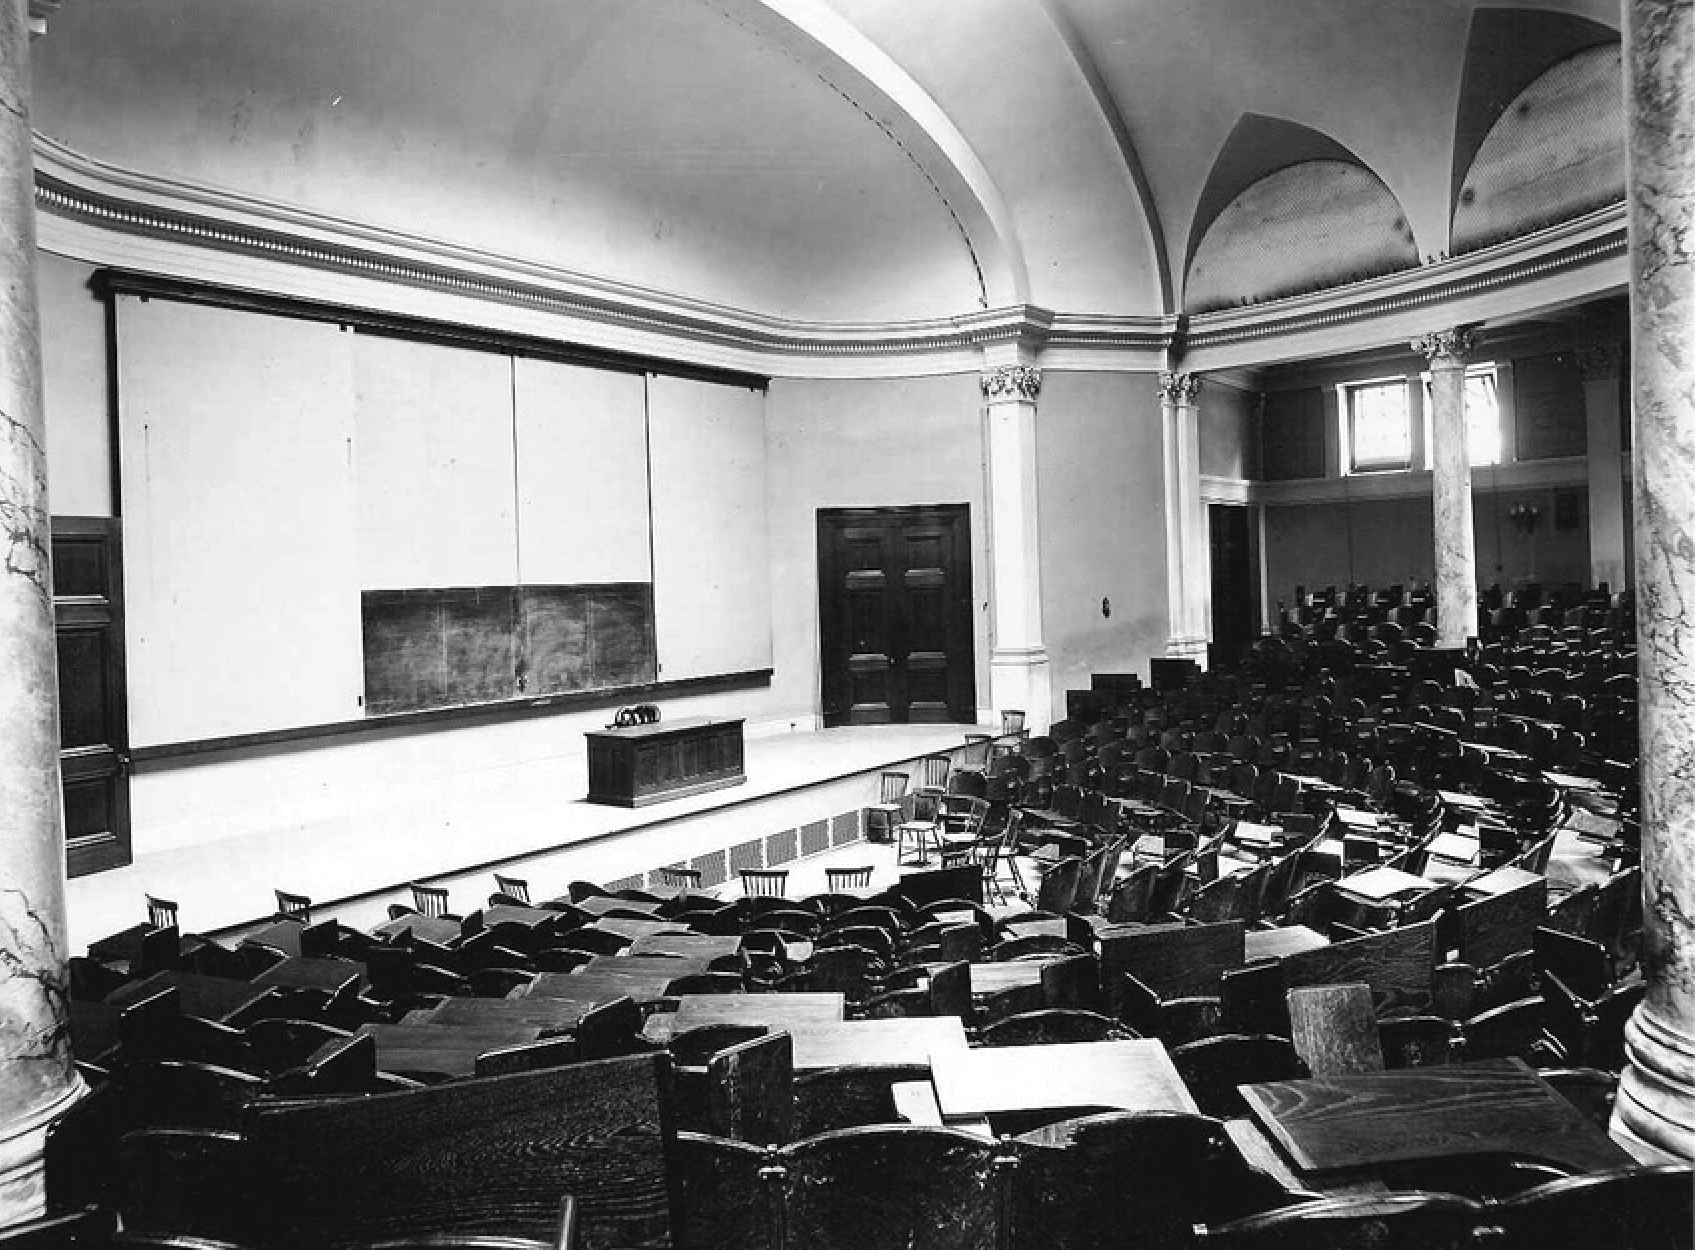
\includegraphics[width=\textwidth]{Graphics/Sabine-Fogg.png}
\caption{Fogg Art Museum lecture hall}
\label{fig:fogg}
\end{figure}

\clearpage

\section{Wallace C. Sabine: l'alba dell'acustica architettonica}

Nonostante l'acustica sia stata per millenni presa in considerazione durante il
processo architettonico, la \emph{fisica acustica} ha ottenuto una base
scientifica solida solo nei primi del novecento, grazie agli studi di
\ws\footcite{ws:rev}. Dopo Sabine il tempo di riverbero può essere descritto,
misurato, previsto. Tutte le conosenze attuali, anche l'opera di
\ms\footcite{ms:rev62, ms:rev64}, sono frutto dei suoi studi

\begin{quote}
  The following investigation was not undertaken at first by choice, but devolved
  on the writer in 1895, through instructions from the Corporation of Harvard
  University to propose changes from remedying the acoustical difficulties in
  the lecture-room o the Fogg Art Museum, a building that had just been completed.
  About two years were spent in experimenting on this room, and permanent changes
  where then made. Almost immediately afterward it become certain that a new
  Boston Music Hall would be erected, and the questions arising in the
  consideration of its plans forced a not unwelcome continuance of the general
  investigation\footcite{ws:rev}.
\end{quote}

Curioso notare che tutto il suo lavoro nasca dalla necessità di dover correggere
l'acustica di una sala universitaria adibita a \emph{lecture room}.
Spinto da una mancanza di informazioni e studi pregressi, \ms~ ha costruito una
ricerca organica, con seri problemi da risolvere.

\begin{quote}
  In order that hearing may be good in any auditorium, it is necessary that the
  sound should be sufficiently loud; that the simultaneous components of a
  complex sound should maintain their proper relative intensities;
  and that the successive sounds in rapidly moving articulation, either of speech
  or music, should be clear and distinct, free from each other and from extraneous
  noises. Thesethree are the necessary, as they are the entirely sufficient,
  conditions for good hearing\footcite{ws:rev}.
\end{quote}

Una tripletta di problemi minimi da comprendere e risolvere per rendere accettabile
il riverbero acustico di un ambiente.

\subsection{Loudness}

\ws~ introduce il concetto di propagazione del suono in forma emisferica, che
si riduce proporzionalmente all'aumentare della distanza. Anche con l'aumento
del pubblico, che occupa dunque maggior spazio nella stanza, il suono perde
intensità più rapidamente, assorbito. La parte superiore della propagazione si
muove libera, non affetta da assorbimenti. I primi accorgimenti: elevare
l'oratore ed alzare da terra le file posteriori. Questa soluzione rimanda
inequivocabilmente ad una forma molto conosciuta: il teatro Greco. Un tetto a
coprire la struttura incrementerebbe l'intensità media, soprattutto dei suoni
sostenuti nel tempo, e ne bilancerebbe la resa tra fronte e fondo sala.

\begin{quote}
  The problem of calculating the loudness at different parts of such an
  auditorium is, obviously, complex, but it is perfectly determinate, and as
  soon as the reflecting and absorbing power of the audience and of the various
  wall-surfaces are known it can be solved approximately\footcite{ws:rev}.
\end{quote}

Per la prima volta non parliamo di riverbero, al singolare, ma molti per ogni
ambiente che descriviamo.

\subsection{Interferenze e Risonanze}

Avendo suoni diretti e riflessi che viaggiano nello stesso ambiente, ci si può
imbattere in somme di ampiezza ma anche in cancellazioni se le fasi sono
rispettivamente congruenti o inverse. Tutto questo accade in relazione al suono
emesso, alla sua altezza, che variando, varia l'intero stato di equilibrio,
l'inntero stato di interferenza.

C'è un altro fenomeno che occorre in queste circostanze, in relazione con
l'intererenza, ovvero la risonanza.

\begin{quote}
  The word \emph{resonance} has been used loosely as synonymous with
  \emph{reverberation}, and even with \emph{echo}, and is so given in some of
  the more voluminous but less exact popular dictionaries. In scientific
  literature the term has received a very definite and precise application to
  the phenomenon, wherever it may occur, of the growth of a vibratory motion of
  an elastic body under periodic force stimed to its natural rates of vibration.
  A word having this significance is necessary; and it is very desirable that
  the term should not, even popularly, by meaning many things, cease to mean
  anything exactly\footcite{ws:rev}.
\end{quote}

\subsection{Riverberazione}

Il fenomeno definito riverbero, il processo delle rilessioni multiple, tra le
superfici di un luogo, è alla base della mal comprensione presente nel luogo di
studio. Il riverbero consiste inoltre in una massa di suono che riempie uno
spazio della quale è impossibile cogliere ed analizzare la singola riflessione
e la cui durata. La misurazione temporale diventa quindi fondamentale, oggi
piuttosto scontata per misurazioni fisiche di ordine infinitamente piccole, ma
per \ws~ non era proprio così.

Il percorso di misurazione del tempo di decadimento del \emph{suono residuo}
evidenzia a \ws~che ci sono due e due variabili soltanto di un luogo  ad
influire sul risultato cronometrico: la forma della stanza, inclusa la
dimensione; i materiali, incluso l'arredamento.

Il culmine di questo studio, oltre a dimostrare che esiste una correlazione tra
la quantità di superficie assorbente (pareti, sedute, persone) e la qualità di
percepimento del suono in una stanza, è lo sviluppo di una formula in grado di
ricavare il tempo in cui il suono decade fino ad una situazione di equilibrio.

Parliamo di \emph{RT60} ovvero il tempo in cui il suono (riverberato) decade di
$60 dB$.

\begin{equation}
RT60 = \frac{24(\ln{10})V}{c s_a}
\end{equation}

Di cui:
\begin{compactitem}
\item $V$ è il volume della stanza
\item $c$ è la velocità del suono
\item $s_a$ è il valore di assorbimento totale espresso in Sabins
\end{compactitem}

Possiamo calcolare i \emph{Sabins} sommando l’area totale delle pareti (per
esempio 4 mura + 1 soffitto e 1 pavimento) e moltiplicandola per il coefficiente
di assorbimento (ovviamente il coefficiente può essere diversificato per i
diversi materiali delle pareti). Da notare che il coefficiente è un valore che
varia tra 0 (minimo assorbimento) e 1 (massimo assorbimento).

L’articolo è considerato un capolavoro di acustica applicata e ha avuto una
grande influenza sullo sviluppo della scienza del suono e sulla progettazione
degli spazi sonori.

\subsection{Echi di Sabine}

Ci sono innumerevoli spunti di riflessione tra le pagine dei testi di \ws\footcite{ws:rev},
dai quali, agli scopi di una corretta implementazione digitale del riverbero e
soprattutto agli scopi di un corretto utilizzo musicale, possiamo ricavare:

\begin{compactitem}
  \item La durata del suono residuo ascoltabile in un ambiente è approssimativamente
  uguale in ogni punto dello spazio.
  \item La durata del suono residuo ascoltabile in un ambiente è approssimativamente
  indipendente dalla posizione della sorgente.
\end{compactitem}

Sono questi due presupposti fondamentali, sui quali cercheremo di costruire un
pensiero musicale prima ancora che uno strumento musicale, quale il riverbero
digitale può essere.

% % !TEX TS-program = pdflatex
% % !TEX root = ../tesi.tex
%
% %************************************************
% \chapter{Acustica}
% \label{chp:Acustica}
% %************************************************
%
% Questo capitolo affronta il processo della produzione, dispersione e percezione dell'onda sonora. Il campo della scienza che si occupa degli studi relativi alla fisica del suono si chiama \emph{acustica}, i cui primi passi sono stati mossi già dai primi \textit{pitagorici} portando innovazione ancora oggi. Di studi più recenti sulla percezione dell'evento sonoro da parte dell'uomo se ne occupa invece la \textit{psicoacustica}.
%
% \section{Il Suono}
%
% Per sintetizzare un riverberatore è necessario prima comprendere, dal punto di vista fisico, cosa accade nel momento in cui un suono viene generato e del suo comportamento nello spazio circostante.
%
% Per \textbf{\textit{suono}} intendiamo un'alterazione di pressione, velocità e posizione delle particelle, propagata in un mezzo elastico, o la sovrapposizione di tali alterazioni.
% Parlando di suono ci riferiamo anche alla percezione definita dal nostro sistema uditivo delle alterazioni sopracitate (H. F. Olson - Elements of acoustical engineering - 1957 pag2).
%
% Il suono è prodotto quando il mezzo di propagazione (nella maggior parte dei casi l'aria)
% è messo in vibrazione da un qualsiasi evento di natura meccanica, per esempio, l'oscillazione di una corda o il battere di un oggetto su una superficie solida  (Harry f.olson - Elements of acoustical engineering - 1957 pag 2).
%
% Queste vibrazioni, propagate in modo sferico, raggiungono il nostro orecchio avente la funzione di trasduttore (trasforma l'energia cinetica in impulsi elettrici) risultando nella nostra percezione dell'evento sonoro.
%
% \subsection{Caratteristiche}
% Le caratteristiche principali, sempre dal punto di vista fisico del suono percepito sono dunque:
% \begin{itemize}
%       \item \emph{Periodo}:
%       Il tempo di completamento di un ciclo (ovvero quando, un segnale periodico esprime tutti i suoi valori ricorrenti) espresso in secondi
%       \item \emph{Frequenza}:
%       il numero di cicli in 1 secondo, si esprime in hertz
%       \item \emph{Lunghezza d'onda}:
%       la distanza tra 2 massimi consecutivi, si esprime in metri
%       \item \emph{Ampiezza}:
%       massima escursione dal punto di equilibrio
%       \item \emph{Velocità dell'onda}:
%       velocità di movimento del fronte d'onda nel mezzo, si esprime in metri al secondo.
% \end{itemize}
% (D. Davis - Sound System Engineering - 2013 pag 171)
% \bigskip
%
% Ovviamente queste caratteristiche non sono universali ma dipendono da fattori ambientali che ne definiscono i valori. Due eventi sonori, di partenza identici, non verranno percepiti ugualmente al variare delle condizioni esterne.
% Queste condizioni che influiscono sul suono sono:

\section{Brevi Nozioni di Acustica}

In questa sezione saranno esposti, in maniera più o meno breve, i principi di carattere fisico e 
percettivo che verranno utilizzati nell'implementazione finale.
Il campo della scienza che si occupa degli studi relativi alla fisica del suono si 
chiama \emph{acustica}, i cui primi passi sono stati mossi già dai primi \textit{pitagorici} 
portando innovazione ancora oggi. Di studi più recenti sulla percezione dell'evento sonoro 
da parte dell'uomo se ne occupa invece la \textit{psicoacustica}.

\subsection{Distanza dalla sorgente}

La distanza dalla sorgente sonora è risaputo comportare una diminuzione di
intensità. Dato che l’onda si propaga in modo sferico, segue la legge
dell’inverso del quadrato, comportando una diminuzione di 6 db ad ogni raddoppio
della distanza.

\subsection{Conformazione del gas/Temperatura e densità}

Parlare di temperatura è importante in quanto è un fattore che influisce in
diversi altri fattori presi in esame in questa tesi, ed è inoltre il punto di
partenza della mia ricerca.
Dalla temperatura dipendono infatti la velocità del suono nel mezzo e il valore
di assorbimento atmosferico.
La velocità del suono possiamo calcolarla secondo la seguente formula:

\begin{equation}
C=\sqrt{\frac{\gamma Ps}{\rho}}
\end{equation}
dove

\begin{itemize}
      \item $\gamma$ è il coefficiente di dilatazione adiabatica
      \item $Ps$ è la pressione circostante
      \item $\rho$ è la densità del gas
\end{itemize}

La densità del gas, come per il coefficiente di dilatazione adiabatica, varia a
seconda della temperatura che, data la sua presenza in varie equazioni, diviene
un fattore determinante per la velocità del suono e dunque per le
caratteristiche del riverbero.
Possiamo calcolare la densità tramite la seguente formula (pag 173):
\begin{equation}
\rho = \frac{stp*hg}{(1+t*0.00367)*hg}
\end{equation}

di cui:

\begin{itemize}
      \item $stp$ è la densità del gas a temperatura e pressione standard;
      \item $hg$ è la pressione barometrica del mercurio in centimetri;
      \item $t$ è la temperatura in gradi Celsius;
      \item $0.00367$ è il  coefficiente di dilatazione termica,una costante comune a tutti i gas
\end{itemize}

Possiamo verificare la densità standard dei gas a tabella \ref{tab:dens}

\bigskip
\begin{table}[h]
\centering
\caption{Tabella raffigurante la densità di alcuni gas a \emph{}}
\label{tab:dens}
\begin{tabular}{lcr}
\toprule
Nome del gas & Simbolo & Densità($kg/m^2$) \\
\midrule
Aria & - & 1.2930 \\
Ammonia & $NH_3$ & 0.7710 \\
Nitrogen & $N_2$ & 1.2507 \\
Chlorine & $CI_2$ & 3.2170 \\
Carbon dioxide & $CO_2$ & 1.9760 \\
Hydrogen & $H_2$ & 0.0899 \\
Methane & $CH_4$ & 0.7170 \\
Carbon Monoxide & $CO$ & 1.2500 \\
Oxygen & $O$ &1.4290 \\
Water Vapour & $H_2O$ & 0.804 \\
\bottomrule
\end{tabular}
\end{table}
\smallskip

\subsubsection{Assorbimento atmosferico}
Rappresenta l’effetto di dissipazione dell’energia data dall’azione combinata
di viscosità e calore del mezzo. Perdite di energia aggiuntive sono dovute
all’umidità assoluta. Questo effetto comporta inoltre un aumento
dell’attenuazione con l’aumento delle frequenze.
\begin{figure}[h]
\centering
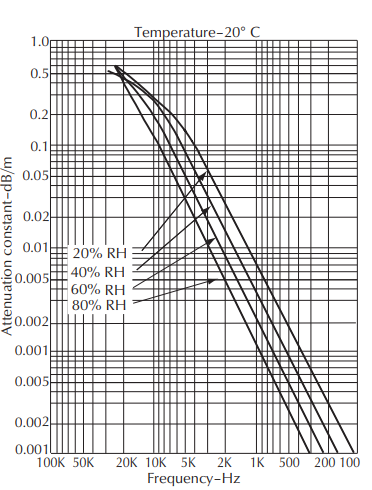
\includegraphics[width=%
0.50\textwidth]{assorbimento}
\caption{Tabella dei coefficenti di assorbimento dell'aria}
\label{fig:assorbimento}
\end{figure}

\subsubsection{Umidità}
Il livello di umidità del gas si riferisce alla presenza o meno di molecole
d’acqua nel mezzo. La sua influenza non è tanto impattante per quanto riguarda
la velocità dell’onda, ma sull’assorbimento acustico totale comportando un
abbattimento di intensità a diverse frequenze.

\subsubsection{Fenomeni di Riflessione}

Le riflessioni sono alla base di ciò che chiamiamo riverbero.
Consistono nella riflessione di un’onda sonora sulle diverse superfici che
circondano l’evento acustico, esse siano pareti oppure oggetti che si interpongono
nella propagazione dell’onda.

Affinché ci sia una riflessione, la superficie riflettente deve necessariamente
essere
più larga di almeno $\frac{1}{4}$ della lunghezza d’onda.
Quando l’oggetto è più piccolo di questa soglia si ha una diffrazione, ovvero
l’onda sonora curva attorno ad esso.

Un altro fenomeno, che possiamo considerare inverso alla riflessione, è \emph{l’assorbimento}.
L’assorbimento è dovuto alle proprietà del materiale che, appunto, al posto di riflettere l’onda assorbono parte dell’energia, trattenendola e restituendo un’onda smorzata.
Più un materiale è assorbente, più sarà rapido il decadimento dell’energia sonora nello spazio fino a tornare in una situazione di stabilità.
La condizione di stabilità sussiste infatti, quando la quantità di energia assorbita è la medesima dell’energia prodotta.

\subsubsection{Fenomeni di Rifrazione}

La rifrazione similmente alla riflessione si ha quando è il mezzo di trasmissione a subire delle variazioni, comportando dunque una differenza nella propagazione in atto. Queste variazioni possono essere, per esempio, temperatura, densità o direttamente un mezzo diverso, basti pensare ad un onda prodotta in aria che incontra una superficie d’acqua.

\section{Psicoacustica}

Altro aspetto da tenere in considerazione è il nostro sistema uditivo. In un sistema lineare in frequenza data in input una lista di frequenze, l’output conterrà le stesse, anche se magari dissimili in ampiezza e fase.
Il nostro apparato uditivo, infatti, a causa di secoli di evoluzione e cambiamenti ha sviluppato dei comportamenti che non lo rendono un sistema lineare, portando dunque a delle inesattezze dal punto di vista percettivo.
Ecco alcuni esempi di fenomeni di non linearità a cui siamo sottoposti:

\begin{itemize}
\item Distorsione armonica:
È la percezione di armoniche superiori di un tono puro. Questa distorsione può essere dovuta ad una pressione eccessiva dell’onda sul timpano;
\item Tono di combinazione:
Detto anche \textit{“terzo suono di Tartini”} è un effetto psicoacustico che comporta nella percezione di un terzo suono, nonostante in input i suoni siano stati solo 2.
La frequenza del tono ricostruito non sarebbe altro che la differenza tra i 2 toni di partenza
\item Curve isofoniche:
Il fenomeno delle curve isofoniche comporta una diversa percezione di ampiezza a per diverse frequenze ma aventi stesso SPL. Per fare un esempio una sinusoide da 1000 Hz a 110 Db SPL ha la stessa percezione di una sinusoide da 3000 Hz ma a 100 Db SPL (ballou - Handbook for Sound Engineers - 2008 - pag 43).
\end{itemize}

\begin{figure}[h]
\centering
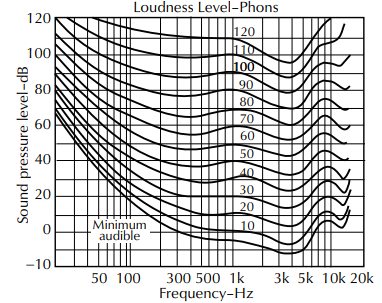
\includegraphics[width=%
0.50\textwidth]{isofoniche}
\caption{Grafico che mostra il comportamento delle curve isofoniche}
\label{fig:isofoniche}
\end{figure}
Questo è anche il motivo per il quale siamo più sensibili nella banda intorno ai 4 KHz, comportando dolore nell’ascoltatore se sottoposto a db elevati.
\subsubsection{Percezione della distanza}
Più interessante ai fini della tesi è la percezione della distanza, tema chiave nello studio degli spazi e della propagazione del suono.
È noto che, duplicata la distanza tra fonte sonora e ascoltatore, il SPL decade di 6 dB.
Nonostante questo, affinché abbiamo la percezione della duplicazione della distanza c’è bisogno della diminuzione di almeno 20 dB (j. Blauert spatial hearing).

Un elemento che però ci permette di comprendere quando una fonte è lontana è la sua composizione spettrale, infatti, a causa dell’assorbimento dell’aria (del mezzo per essere più precisi) le frequenze alte saranno assorbite maggiormente, comportando una presenza più elevata di basse frequenze.

Per questo, in modo tale da replicare distanza e vicinanza dalla fonte sonora, oltre a questi accorgimenti è da tenere in considerazione il rapporto tra suono diretto e riverberato.
In un ambiente reale infatti, è proprio il rapporto tra le due sorgenti a determinare dove e quanto è distante un evento sonoro.

\section{Spazio}

Come citato poc'anzi quando si parla di suono bisogna considerare quindi lo spazio e il mezzo in cui l'onda si propaga.
Possiamo classificare gli spazi in diverse categorie, le principali sono (Davis - Pag 178):
\begin{itemize}
\item Free Field:
È definito così uno spazio uniforme, libero da ostacoli che potrebbero produrre delle riflessioni o rifrazioni e non contaminato da sorgenti sonore estranee.
Esempi di questo tipo sono le sale anecoiche (senza eco),camere particolari il cui scopo è quello di ridurre al minimo le riflessioni delle onde, utili per eseguire test precisi su apparecchiature audio.
\item Reverberant field:
È uno spazio chiuso, con pochissimo assorbimento acustico, in cui la pressione sonora è uniforme in ogni punto e le onde si propagano allo stesso modo in tutte le direzioni.
Caratteristiche di questo tipo possiamo trovarle in luoghi come camere vuote o cavità.
\item Semireverberant Field:
È il tipo di spazio più comune che possiamo incontrare, nel quale l’energia è sia assorbita che riflessa. L’energia si muove in più direzioni ma è comunque percepibile il punto di origine della fonte di generazione dell’evento sonoro.
\end{itemize}

\subsection{Risposta all'impulso}

Al giorno d’oggi conosciamo una tecnica in grado di eseguire una fotografia delle caratteristiche acustiche in grado di descrivere come il suono si propaga da un punto di emissione ad un ricevitore.

Parliamo di \textit{Risposta all’impulso} ovvero del modello fisico-matematico di un sistema lineare, non dipendente dal tempo, composto solo da un input ed un output\footcite{af:book}.

Le informazioni contenute sono sia relative al dominio del tempo, ad esempio riflessioni e ritardi nella propagazione che, relative al dominio della frequenza, comportando quindi modifiche dal punto di vista spettrale.

Il sistema utilizzato viene detto \textit{Black box} che, come detto in precedenza è composto da un singolo input ed un singolo output. All’interno di questa black box gli elementi che concorrono all’acquisizione dei dati matematici dello spazio che si vuole registrare sono:
\begin{itemize}
\item Un generatore di segnale: Tipicamente un pc;
\item Un amplificatore di segnale;
\item Un diffusore di segnale: il quale riproduce il segnale nello spazio in modo omnidirezionale;
\item Un ricevitore: un microfono anch’esso omnidirezionale, in quanto vogliamo escludere la direzionalità dallo studio.
\end{itemize}
Per misurare quindi la risposta all'impulso riproduciamo il segnale attraverso l’altoparlante nello spazio e contemporaneamente registriamo come, quel segnale, si propaga in quel determinato spazio e in quelle determinate condizioni, attraverso il microfono.

Il segnale originale consiste in uno sweep esponenziale il quale parte dalla frequenza $f_1$, termina a frequenza $f_2$ in $t$ secondi.

Il segnale riverberato conterrà al suo interno componenti spettrale non presenti nell’originale, che corrispondono alla risposta lineare in frequenza dello spazio.
Attraverso un processo di convoluzione, ampiamente spiegato e perfezionato dal prof. A Farina, siamo in grado di restituire la risposta all'impulso del sistema lineare.

È da tenere conto che però una singola registrazione non è in grado di descrivere tutto lo spazio. La risposta all’impulso, come già detto, è relativa soltanto al punto in cui è posizionato il ricevitore e soltanto per il punto da cui è emesso il suono. Per la mappatura dello spazio per restituire un'immagine fedele dello spazio sono necessarie numerose registrazioni. Come per una fotografia, maggiore è il numero di “pixel”, più definita sarà l’immagine. Per questo è un lavoro che, soprattutto per luoghi ampi, richiede moltissimo tempo e spesso si tende ad effettuare un numero di registrazioni non necessario a restituire un modello fedele.

\subsection{Storia dello studio degli spazi}

Storicamente, in ambito musicale, lo spazio è stato sempre presente ed essenziale durante le performance. Basti pensare agli auditorium greci, dove la conformazione permette sia un rinforzo in termini di ampiezza, ma anche una forte intelligibilità delle parole in modo tale da raggiungere chiaramente tutti i presenti.
Gli ascoltatori, posti ad un'angolazione di circa 120 gradi, ricevevano il suono diretto dall’oratore, seguito delle riflessioni provenienti sia dal pavimento dell’orchestra, che dal retro del palco, anche se con minor intensità.
\begin{figure}[h]
\centering
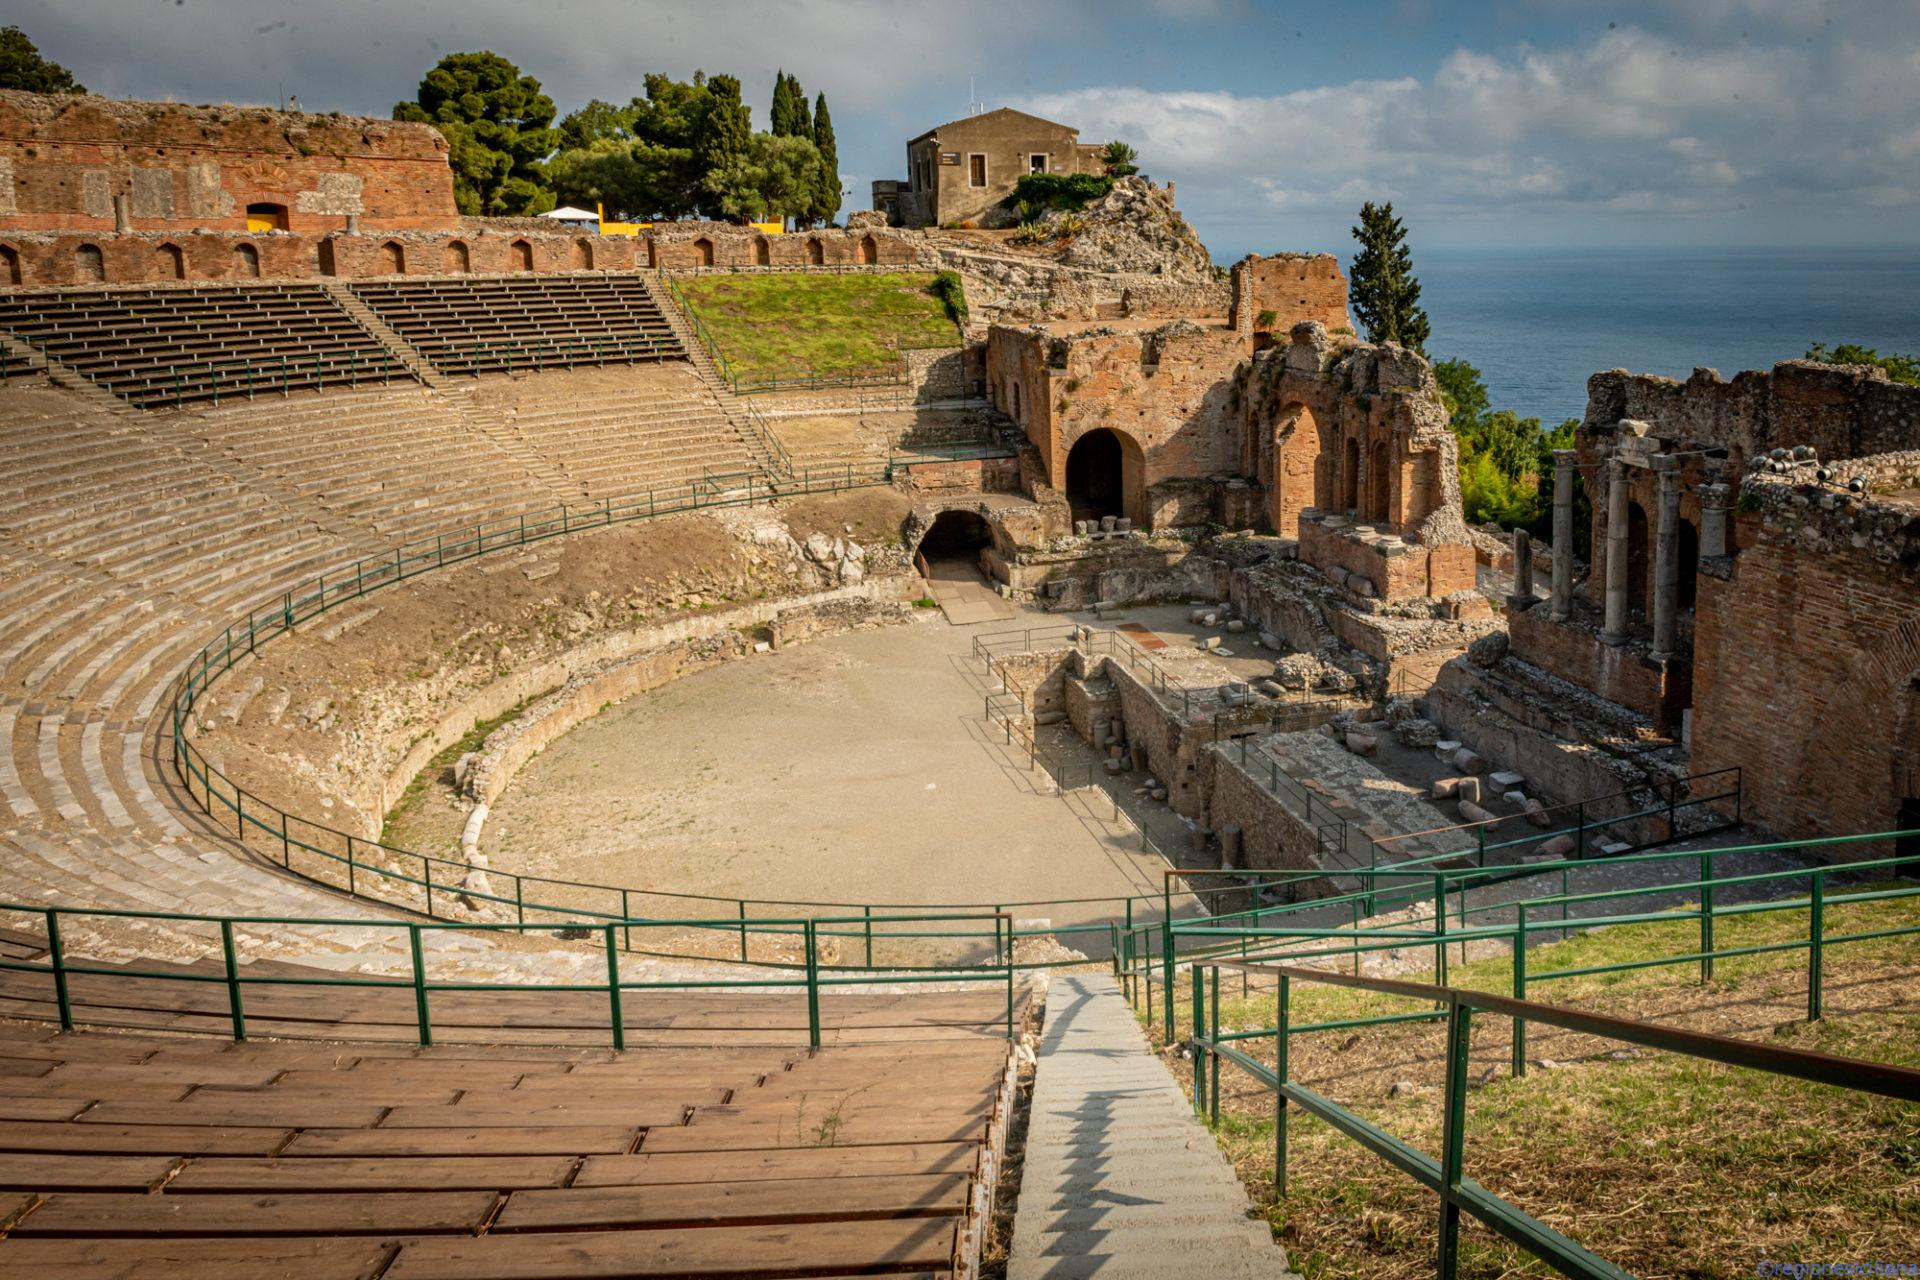
\includegraphics[width=%
0.50\textwidth]{teatrogreco}
\caption{Foto del teatro greco di Siracusa}
\label{fig:teatrogreco}
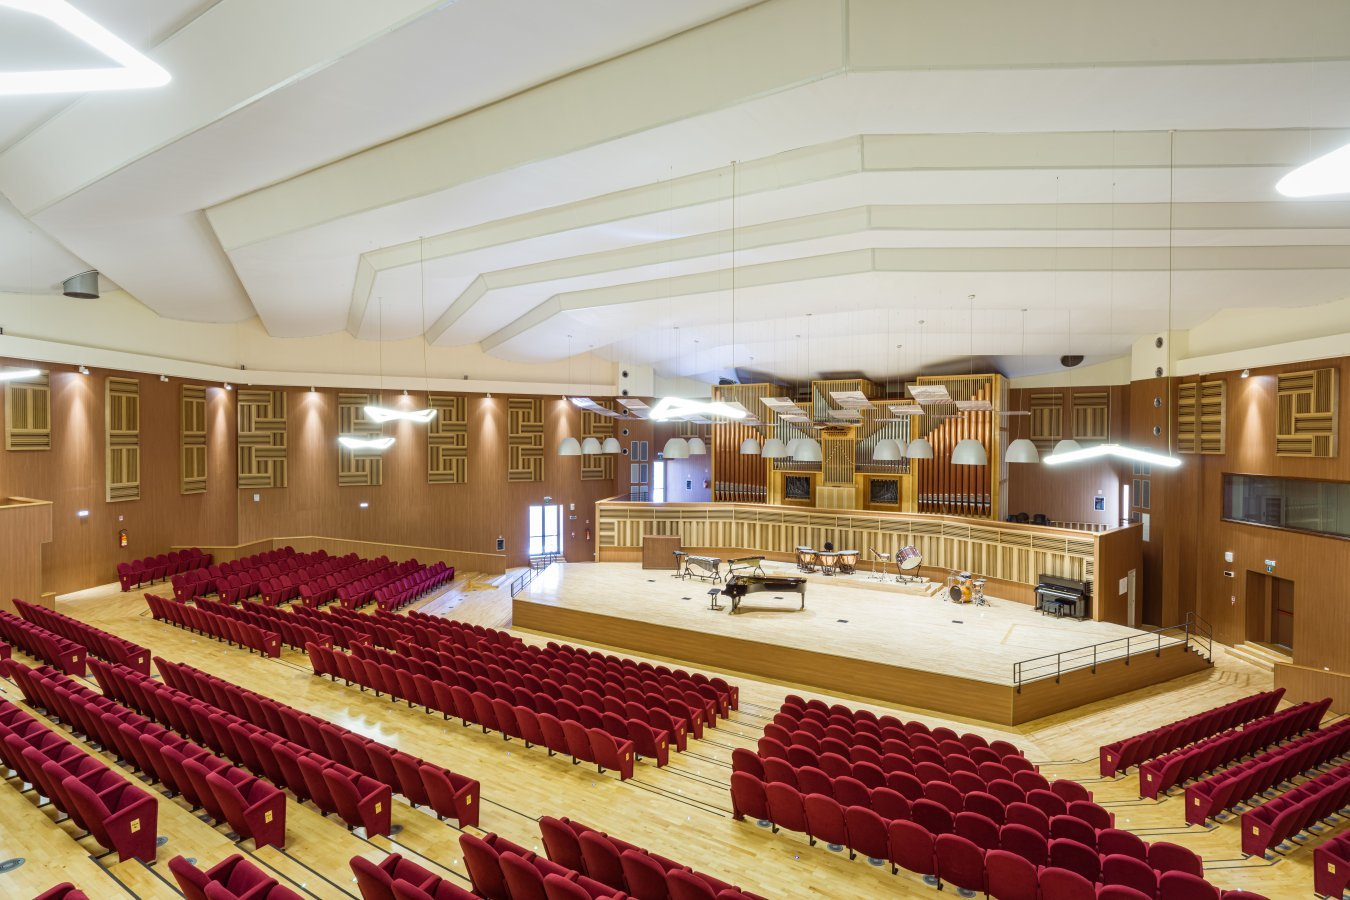
\includegraphics[width=%
0.50\textwidth]{auditorium}
\caption{Foto dell'auditorium Nino Rota del conservatorio di Bari}
\label{fig:auditorium}
\end{figure}
Il palco, inoltre, aveva un’ altezza compresa tra 1m e 3.6m, comportando una differenza nell’angolo di incidenza del suono diretto (Auditorium Acoustics and Architectural Design Di Michael Barron).
Infine, un altro accorgimento degli architetti greci, i quali avevano scoperto le proprietà di assorbimento, era il posizionamento tra le sedute di vasi contenenti ceneri, i quali avevano lo scopo di assorbire l’energia sonora che sarebbe stata riflessa indietro verso il palco.
\bigskip
Un’altro esempio in cui vediamo lo spazio come protagonista, è il caso degli organi, in cui il luogo è la vera e propria cassa armonica dello strumento.
L’acustica dell’organo è fortemente legata alla sua ubicazione, infatti, a differenza di altri strumenti musicali i quali possono essere spostati e trasportati, per l’organo non è possibile. Inoltre i luoghi provvisti di organo sono spesso molto riverberanti, come ad esempio le chiese e i teatri, e questo concorre alla definizione timbrica dello strumento
\begin{figure}[h]
\centering
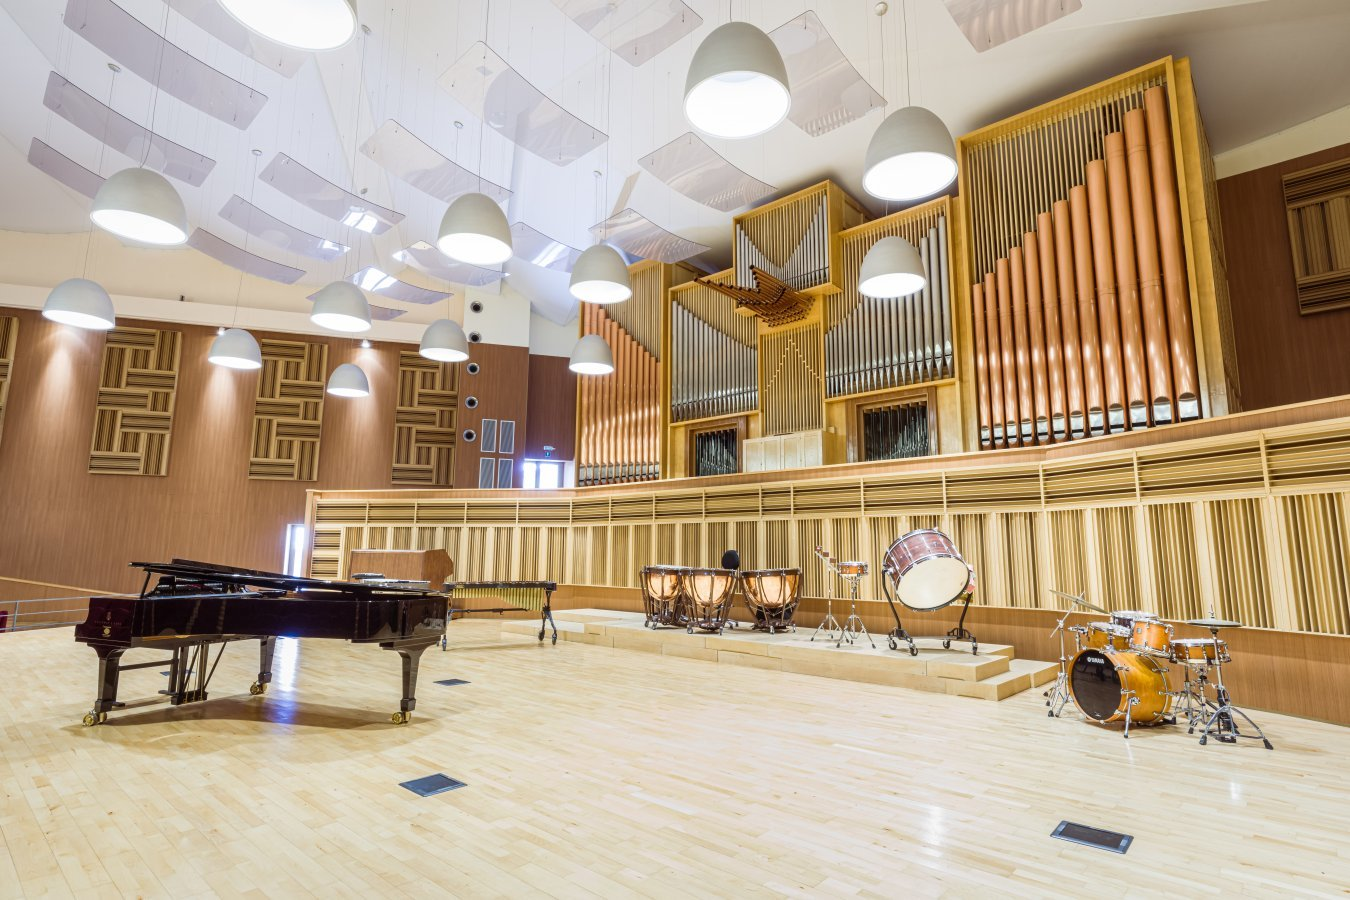
\includegraphics[width=%
0.50\textwidth]{organo}
\caption{Foto dell'organo presente nell'auditorium N.Rota}
\label{fig:organo}
\end{figure}
\subsubsection{Lo spazio come parametro}
Si è dovuto attendere però circa gli anni 60 affinchè lo spazio diventasse un vero e proprio parametro compositivo.

\emph{“Gesang der Jünglinge"} di Karlheinz Stockhausen è un’opera importantissima per l’epoca in cui è stata composta. Il brano, nato pentafonico e successivamente ridimensionato in quadrifonia, rappresenta l’avanguardia del serialismo integrale. Come accennato in precedenza, questo lavoro è il primo esempio in cui vediamo la gestione dello spazio come parametro compositivo, al pari di ampiezza, altezza e timbro.
Gli altoparlanti, disposti circolarmente attorno agli ascoltatori, creano uno spazio in cui immergersi permettendo complessi movimenti tra gli stessi.
Vengono infine introdotti termini quali “Intervallo spaziale” e “Accordi di spazio”.

\section{Architetture di riverberazione artificiale}

Non esiste un unico modo di ricreare un riverbero ma, come è possibile intuire, negli anni si sono sviluppate differenti tecniche per raggiungere questo scopo.
Innanzitutto bisogna definire 2 categorie di principali:

\begin{itemize}
\item Analogici
\item Digitali
\end{itemize}

Le tecniche di riverberazione analogica, non presentano processi di trasformazione digitale del segnale, senza quindi utilizzare operazioni matematiche al loro interno.
Di questa categoria citiamo:

\begin{itemize}
\item Riverberi Elettromeccanici: Questa tipologia di riverbero utilizza un elemento riverberante all’interno del proprio circuito. Due esempi degni di nota sono gli \emph{“spring reverb” e “plate reverb”} che, come suggerisce il nome, utilizzano molle, nel primo caso e placche metalliche, nel secondo, per simulare l’effetto del riverbero sul segnale originale. In poche parole l’elemento riverberante fungeva da ponte tra l’entrata e l’uscita del sistema, modificando le proprietà acustiche del segnale in input.
\item Camere riverberanti: Questa tipologia si serve di uno spazio realmente esistente al cui interno è presente un diffusore ed un microfono. Il segnale originale viene emesso dall’altoparlante che, diffondendosi nello spazio circostante, acquisisce un riverbero non presente all’origine. Il risultato viene poi successivamente registrato dal microfono, conservando le nuove proprietà.
\end{itemize}

Per quanto riguarda le tecniche di \emph{riverberazione digitale}, parliamo di processi in cui il segnale originale, digitalizzato, subisce modifiche tramite calcoli matematici. La tecnica più diffusa è quella del riverbero algoritmico che prevede una serie di \textit{somme, prodotti e delay}. Successivamente parleremo in modo più dettagliato di questa tecnica.

Degna di nota è un’ulteriore tecnica digitale, diffusasi negli ultimi anni, che utilizza la \emph{convoluzione}. Senza entrare troppo nei dettagli la convoluzione è un processo matematico di moltiplicazione tra due segnali che avviene campione per campione. La convoluzione è utilizzata tra il segnale originale e la risposta all’impulso di uno spazio esistente, producendo in output un segnale avente le medesime caratteristiche di quest’ultimo.

\section{Natural Sounding Schroeder Reverberation}

La base da cui partiamo per la realizzazione del riverbero algoritmico sono gli studi fatti da Manfred R. Schroeder riportati nel suo articolo “Natural Sounding Artificial Reverberation” pubblicato nel 1962 in seguito agli esperimenti condotti a Murray Hill, presso i Bell Laboratories.

Manfred Robert Schroeder è stato un fisico tedesco conosciuto per i suoi studi su acustica, telecomunicazioni e computer grafica. Nasce nel 1926, ad Ahlen in Germania e già da giovane mostra interesse nell’elettronica e nelle telecomunicazioni. Dopo un periodo di interruzione dallo studio a causa del suo reclutamento durante la Seconda Guerra mondiale, Manfred conclude i suoi studi sotto la tutela del prof Erwin Meyer, un’ autoritá nel mondo dell’acustica.
In seguito alla sua laurea, il suo lavoro è stato lodato dall’amministrazione dei Bell Laboratories, i quali gli hanno offerto un impiego nella divisione di ricerca a Murray Hill, New Jersey. Da lì in poi ha proseguito le sue ricerche spaziando dalle telecomunicazioni all’acustica conseguendo numerosi riconoscimenti in tutto il mondo.

Il sopracitato laboratorio Bell Labs è inoltre importante da citare in quanto, oltre ad essere un’ istituzione nel campo delle telecomunicazioni, è un eccezionale esempio di collaborazione e progresso. Il laboratorio era un apparato di Bell System, una società telefonica che ha operato in America fornendo servizi a livello nazionale. Lo scopo del laboratorio, dunque, era quello di fornire nuove tecnologie all’avanguardia nel campo delle telecomunicazioni. Da ciò si può facilmente intuire innanzitutto il grande capitale e le tecnologie messe a disposizione dei ricercatori, tra cui Schroeder, e dell’ambiente ricco di menti portate all’innovazione tecnologica.

\subsection{Analisi}

Come detto, partiró dall’analisi fatta da Schroeder per la progettazione del riverbero.
In quel periodo, parliamo del 1962, gli studi e le tecnologie in grado di sintetizzare un riverbero erano acerbe.
Le tecniche più diffuse all’epoca, le quali partivano delay creati su nastro magnetico, disco o molle, non producevano un effetto fedele al riverbero naturale per 2 aspetti principali:

\begin{itemize}
\item La loro risposta, sia in frequenza che in ampiezza, non era piatta, comportando una “colorazione” nel risultato, soprattutto se solo una piccola parte del segnale diretto veniva missato al segnale riverberato.
\item La densità degli echi non era sufficiente a creare un risultato credibile. La ricerca di Schroeder ci mostra che circa 1000 echi al secondo è un risultato accettabile per un riverbero sintetico. Consideriamo che in un ambiente reale le riflessioni sono infinite, ma questo sarebbe un risultato quasi impossibile da raggiungere
\end{itemize}

Nel suo articolo “Natural Sounding Artificial Reverberation”, M. R. Schroeder mostra il suo approccio alla risoluzione per le problematiche sopracitate.

In primo luogo per ovviare al primo problema è necessario creare una linea di ritardo con feedback che abbia una risposta piatta in ampiezza e frequenza.
Utilizzando lo schema proposto da schroeder, abbiamo un dispositivo (informatico, in questo caso) incaricato di restituire un singolo eco, dopo un ritardo temporale ($t$)

\begin{figure}[htp]
\centering
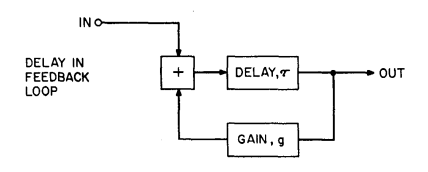
\includegraphics[width=%
0.50\textwidth]{dfl}
\caption{Delay all'interno di un feedback}
\label{fig:dfl}
\end{figure}

Dato che l'obiettivo è quello di produrre un elevato numero di echi a partire da un numero contenuto di oggetti, inseriamo dunque la linea di ritardo in un feedback avente come moltiplicatore $(g) < 1$.
Il risultato sarà un segnale che decade di $g$ volte ad ogni ciclo.

\begin{figure}[htp]
\centering
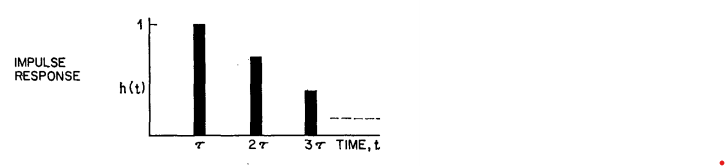
\includegraphics[width=%
0.60\textwidth]{dflir}
\caption{risposta in ampiezza}
\label{fig:dflir}
\end{figure}

La sua risposta in frequenza invece, presenta in modo periodico picchi e valli sullo spettro, aventi come valori rispettivamente $(1+g)$ e $(1-g)$. L’autore, data la somiglianza ad un pettine, rinomina il ciclo sopra descritto \emph{Comb Filter}, e così mi riferirò al medesimo d’ora in avanti.

\begin{figure}[htp]
\centering
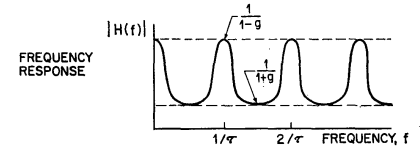
\includegraphics[width=%
0.50\textwidth]{dflspectrum}
\caption{}
\label{fig:dflspectrum}
\end{figure}

Questo comportamento del filtro comporta però una certa non esattezza in termini di spettro che Schroeder cerca di evitare, raffinando l’algoritmo tramite successive integrazioni.
La soluzione proposta dall’autore e Logan è il missaggio del suono diretto moltiplicato per $(-g)$ e il suono riverberato moltiplicato per $(1-g^2)$. Questo comporta una risposta piatta per tutte le frequenze. Il filtro risultante, chiamato \emph{All Pass Filter}, è descritto secondo il seguente schema e per le successive integrazioni, viene utilizzato come unità riverberante di base.

\begin{figure}[htp]
\centering
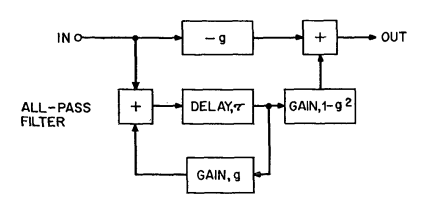
\includegraphics[width=%
0.50\textwidth]{apf}
\caption{All Pass filter di Schroeder}
\label{fig:apf}
\end{figure}

Per risolvere la problematica della densità degli echi, la soluzione di schroeder è quella di connettere in serie più riverberatori, in modo tale che la densità cresca in modo frattale per ogni unità connessa. Dato che abbiamo risolto il problema di una possibile colorazione del filtro, possiamo non preoccuparci che questo avvenga per una connessione in serie.

\begin{figure}[htp]
\centering
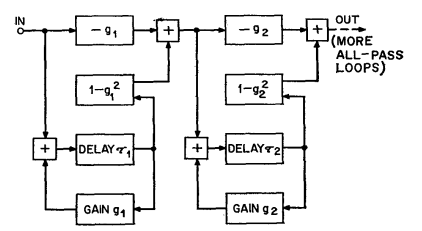
\includegraphics[width=%
0.50\textwidth]{apfseq}
\caption{sequenza di 5 All Pass}
\label{fig:apfseq}
\end{figure}

La densità che si cerca di raggiungere, ovvero quella di circa 1000 echi al secondo, è facilmente raggiungibile con 5 riverberatori in serie (il numero prodotto è di circa 810). A differenza di Schroeder abbiamo a disposizione molte più risorse, in termini di potenza di calcolo infatti possiamo serializzare molti più riverberatori e raggiungere un numero di riflessioni elevatissimo.

Successivamente, avendo constatato l’efficienza del riverberatore All Pass, Schroeder cerca di implementare alcune caratteristiche della riverberazione naturale.

Esse sono:

\begin{itemize}
\item Missaggio del suono diretto con il suono riverberato, senza alterare la struttura di All Pass;
\item Inserimento di un leggero sfasamento temporale tra, appunto, il segnale diretto e il segnale riverberato, dato che come sappiamo, il suono diretto raggiunge l’ascoltatore prima delle riflessioni;
\item La dipendenza alle frequenze del tempo di riverbero;
\end{itemize}

Il segnale non riverberato restituito dalla sequenza di all-pass risulta parecchio ininfluente, per questo Schroeder consiglia di moltiplicare per ($-g$) e sommare il segnale diretto proprio con questa serie, come illustrato in figura \ref{fig:apfmix}.

\begin{figure}[htp]
\centering
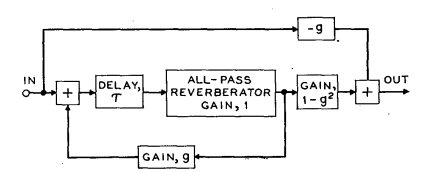
\includegraphics[width=%
0.50\textwidth]{apfmix}
\caption{sequenza di All Pass con aggiunta di segnale diretto}
\label{fig:apfmix}
\end{figure}

Il box chiamato \emph{“All-pass reverberator”} contiene, come detto, la serie di All Pass, inserito all’interno di un ulteriore feedback loop.
Da notare il delay iniziale, il quale permette un ritardo rispetto al suono diretto, rifornendo anche il secondo punto.

\bigskip

Un ultimo aspetto da considerare dell’articolo,  è l’utilizzo combinato di filtri Comb e All-pass per ricercare, al contrario dell’obiettivo originale, una risposta frequenziale altamente irregolare, come nel caso delle stanze reali.
In seguito agli esperimenti condotti ai Bell Telephone Laboratories, in cui si è scoperto che ad alte densità di riflessioni le irregolarità sono impercettibili, si è pensato di ricostruire l’algoritmo in modo tale da ricreare le condizioni di una stanza reale.
Lo schema è raffigurato in figura \ref{fig:comballpass}
\smallskip

\begin{figure}[htp]
\centering
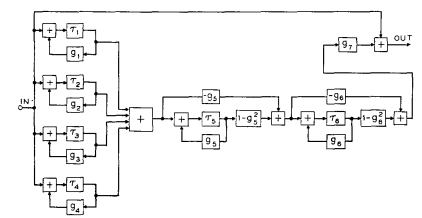
\includegraphics[width=%
0.60\textwidth]{comballpass}
\caption{Configurazione Comb-All Pass}
\label{fig:comballpass}
\end{figure}

Questa nuova configurazione conformazione prevede:
\begin{itemize}
\item Un certo numero di Filtri Comb, aventi tempi di delay incommensurabili oppure primi, connessi in parallelo. Questi filtri produrranno le cosiddette “Early reflections";
\item Un certo numero di All-Pass connessi in serie, in modo tale da incrementare la densità degli echi.
\item Al tutto verrà aggiunta una quantità di segnale diretto come nelle precedenti iterazioni.
\end{itemize}

\section{Moorer's Business}
Un successivo studio sulla simulazione digitale dei riverberi è stato condotto da \emph{James A. Moore} intorno al 1979, pubblicando i suoi risultati  su Computer Music Journal ,Vol. 3, No. 2.
L’articolo, intitolato \emph{“About this Reverberation Business”}, tratta di ulteriori integrazioni e accorgimenti che possono essere applicati durante lo sviluppo di un riverbero.

L’autore, infatti, partendo dalla letteratura già presente, tra cui gli articoli di Schroeder e J.Chowning, sperimenta nuovi algoritmi, rendendo più snelli i precedenti, sempre tendendo ad una realisticità del riverbero.

Innanzitutto vengono ripresi i sistemi fondamentali dell’analisi di Schroeder, vale a dire, il filtro Comb (visto in figura \ref{fig:dfl}) e il filtro All Pass (visto in figura \ref{fig:apf}). Quest’ultimo in una seconda versione caratterizzata da una singola moltiplicazione, a fronte delle 3 precedenti, rendendolo più sostenibile a livello di computazione.

\begin{figure}[htp]
\centering
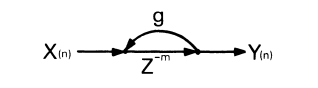
\includegraphics[width=%
0.60\textwidth]{combmoorer}
\caption{Filtro Comb di Moorer}
\label{fig:combmoorer}
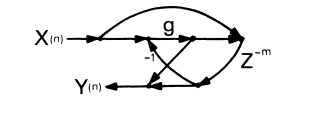
\includegraphics[width=%
0.60\textwidth]{apfmoorer}
\caption{Filtro All Pass di Moorer}
\label{fig:apfmoorer}
\end{figure}

Aventi le seguenti funzioni di trasferimento:
\begin{equation}
T(z) = \frac{g + z^{-m}}{1+gz^{-m}}
\end{equation}
\begin{equation}
T(z) = \frac{z^{-m}}{1-gz^{-m}}
\end{equation}

Osservando la funzione trasferimento dell’All Pass possiamo notare come il coefficiente del numeratore sia in ordine inverso di quello al denominatore, forzando gli zeri ad essere reciproci dei poli, definendo il comportamento All Pass del filtro.

Seguendo il lavoro fatto da Schroeder, per utilizzare i sistemi come riverberatori è necessario utilizzare una combinazione degli stessi.

Le combinazioni sono le medesime viste in precedenza e proposte da Schroeder (fig \ref{fig:apfseq} e \ref{fig:comballpass}). Parliamo dunque di una serie di All Pass nel primo algoritmo e, una cascata di comb filter seguiti da 2 All Pass nel secondo

\begin{figure}[htp]
\centering
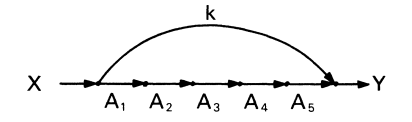
\includegraphics[width=%
0.60\textwidth]{allallpass}
\caption{Filtro Comb di Moorer}
\label{fig:allallpass}
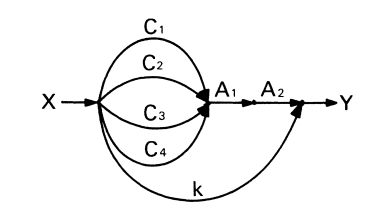
\includegraphics[width=%
0.60\textwidth]{comballpassmoorer}
\caption{Filtro All Pass di Moorer}
\label{fig:comballpassmoorerB}
\end{figure}

\subsection{Problematiche Del riverberatore}

Il riverberatore così ottenuto, però, non rispecchia alcune caratteristiche desiderate, portando ad aberrazioni acustiche non presenti in natura.
Le problematiche riscontrate possono essere riassunte in:

\begin{itemize}
\item riverberazione non ottimale per suoni impulsivi e con transienti molto corti, producendo pattern ritmici composti dagli echi al posto di un riverbero uniforme;
\item riverberazione con un carattere metallico, soprattutto per tempi molto lunghi;
\end{itemize}

A questo punto l’autore considera l’utilizzo di nuove unità riverberanti, ma comunque mantenendo la struttura Comb-All Pass, ritenuta la migliore in termini di risposta.

\subsection{Nuove unità riverberanti}

Nel corso delle sue sperimentazioni Moorer costruisce altre 4 unità riverberanti, alcune molto simili tra di loro in quanto i concetti alla base restano i medesimi. In particolare, l’intuizione dell’autore è stata quella di introdurre un ulteriore filtro all’interno dei feedback.

Lo scopo del filtro, ricollegandoci agli argomenti trattati nei capitoli precedenti, è quello di simulare l’attenuazione delle alte frequenze causate dall’aria. Come già detto, è un coefficiente che, in base a caratteristiche quali umidità e temperatura, sottrae energia alle alte frequenze dello spettro, scurendo quest’ultimo.

\subsection{Nuove unità riverberanti}

Come detto, le unità proposte sono 4, ma una in particolare sembra essere la più efficiente, ovverosia:

\begin{figure}[htp]
\centering
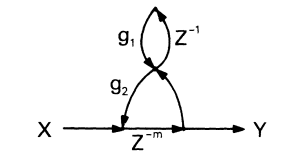
\includegraphics[width=%
0.50\textwidth]{combfiltro}
\caption{Filtro Comb con all'interno un filtro Passa Basso}
\label{fig:combfiltro}
\end{figure}

Come è possibile notare, si tratta di un Comb filter al cui interno è presente un filtro di tipologia Low pass $T(z)$. Il valore di $g_1$ controlla il roll-off del filtro e in seguito troveremo un modo per capire quale valore sarà più conveniente.
All’interno, i valori $g_1$ e $g_2$ seguiranno la condizione di $g_1+g_2<1$ per motivi di stabilità.

La risposta in frequenza, a detta di Moorer,  non sarà in grado di restituire un valore coerente alla realtà, in quanto il singolo filtro Low pass (di primo ordine) è un compromesso per rendere il tutto più efficiente.

Successivamente, nell’articolo viene anche consigliato di tenere in considerazione della modifica dei tempi di delay in base alle caratteristiche dell’aria (temperatura e umiditá), anche se nel testo si fa riferimento a valori standard e non modificabili.
I valori di $g$, dipendenti dall’umidità, sono in seguito esposti grazie agli studi di Moorer nel seguente grafico.
\begin{figure}[h!]
\centering
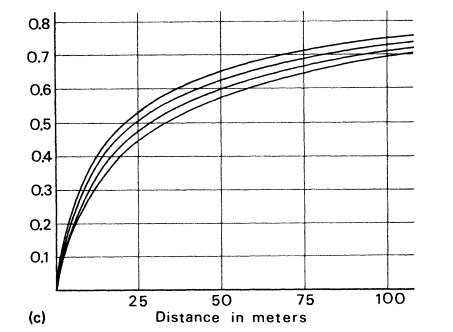
\includegraphics[width=%
0.50\textwidth]{assorbimentomoorer}
\caption{Grafico raffigurante l'andamento del valore di $g$ a causa dell'assorbimento dell'aria}
\label{fig:assorbimentomoorer}
\end{figure}
\bigskip
\subsection{In conclusione}
Moorer conclude la sezione riportando i risultati ottenuti. L’inserimento del filtro permette una miglior riverberazione per i suoni impulsivi, infatti il tempo di ogni eco risulta essere esteso, soprattutto per quanto riguarda le prime riflessioni e nascondendo i vuoti creati dalla bassa densità.
Il risultato sonoro non è particolarmente entusiasmante a detta dell’autore, ma sopperisce ad alcune mancanze delle precedenti iterazioni, rendendo questo sistema il più efficace al momento della scrittura.


% !TEX TS-program = pdflatex
% !TEX root = ../tesi.tex

%************************************************
\chapter{Implementazione}
\label{chp:Implementazione}
%************************************************

% % !TEX TS-program = pdflatex
% % !TEX root = ../tesi.tex
%
% %************************************************
% \chapter{Filtri}
% \label{chp:Filtri}
% %************************************************

\section{Filtri}
Prima di proseguire con l’analisi del riverberatore, c’è bisogno di introdurre il concetto di filtro, oggetto essenziale  per la creazione di quest’ultimo.
Un filtro possiamo definirlo come un dispositivo o rete di dispositivi in grado di separare segnali complessi in base alla loro frequenza. Un filtro, come suggerisce il nome, filtra e permette ad alcune bande di frequenze di essere successivamente emesse oppure escluse dall’output finale.
Alcune caratteristiche presenti nella maggior parte dei filtri sono:
\begin{itemize}
\item Banda Passante:
Banda di frequenze che passa attraverso un filtro e che subisce una perdita di meno di 3 dB;
\item Banda Stoppata:
Banda di frequenze che passa attraverso un filtro e che subisce una perdita di 3 db o più;
\item Frequenza di Taglio
È la frequenza dove il filtro inizia ad eseguire modifiche al segnale, come abbattimenti o enfatizzazioni;
\item Ordine:
È una caratteristica definita dal numero di oggetti all’interno del filtro che concorrono al medesimo risultato, di solito inerenti a scopi di risposta in frequenza del filtro. Se tutti gli elementi sono eterogenei, per esempio passa basso o passa alto, l’attenuazione sarà di 6 db per ordine. Un filtro passa basso del quarto ordine avrà abbattimento di 24 db, ma un passa banda del medesimo ordine ne abbatterà soltanto 12.
\end{itemize}
\medskip
\subsection{Categorie di filtri}
In seguito a queste caratteristiche, passiamo ad eseguire brevi categorizzazioni di filtri in base alla loro componentistica e comportamenti.

Una prima categorizzazione che possiamo eseguire, riguarda la presenza o meno, di componenti che amplificano il segnale. Parliamo di:
\begin{itemize}
\item Filtri Passivi:
Sono filtri che non possiedono amplificatori di segnale, quindi il loro unico scopo è quello di attenuare ciò che li attraversa;
\item Filtri Attivi:
Al contrario, i filtri attivi hanno componenti che permettono l’amplificazione di determinate bande o dell’intero segnale, aggiungendo energia dove necessario.
\end{itemize}

Parliamo di \textbf{equalizzatore} per identificare un dispositivo il cui scopo è quello di sopperire a caratteristiche non gradite, riguardanti ampiezza, frequenza o fase, in modo tale da ricreare la risposta desiderata. Gli equalizzatori, per compiere ciò, sono costituiti da filtri, implementati per svolgere diversi tipi di modifiche.

\section{Funzione di trasferimento}
Prima di proseguire è necessario affrontare in questa sezione un concetto matematico che negli anni ha contribuito allo studio e alla creazione di filtri digitali grazie alla sua estrema versatilità, ovvero le funzioni di trasferimento.

In breve, una funzione di trasferimento è la trasformata della risposta all’impulso di un sistema LTI (Linear Time-Invariant) e riassume in sé le sue caratteristiche.

Si presenta nella seguente forma:
\begin{equation}
H(s)=\frac{\sum_{k=0}^K a_k s^k}{\sum_{n=0}^N a_n s^n}
\end{equation}

È definita tramite una funzione razionale fratta, ovvero una funzione costituita dal rapporto di due polinomi. Ognuno dei due polinomi individua un’equazione rispettivamente di $k$-mo e $n$-mo grado ovvero che ci saranno $k$ soluzioni per il polinomio al numeratore ed $n$ soluzioni per il polinomio al denominatore. Queste soluzioni saranno tutti i valori che rendono nulla la funzione: quelle che azzerano il numeratore si dicono \textbf{zeri} $(-zk)$, quelle che azzerano il denominatore si dicono \textbf{poli} $(-pn)$.

La forma fattorizzata della funzione di trasferimento è la seguente ed è utilizzata per il tracciamento dei grafici di risposta in frequenza dei filtri (detti diagrammi di bode)
\begin{equation}
H(s)=\frac{\prod_{k=1}^k (s+zk)}{\prod_{n=1}^n (s+pn)}
\end{equation}
\bigskip
Semplificando il tutto e ricollegandoci all’argomento principale, è necessario comprendere che poli e zeri corrispondono alla frequenza di taglio del filtro che la funzione di trasferimento rappresenta.
\section{Tipologie di filtro}
Come detto in precedenza, i filtri si distinguono per via della loro architettura alla quale consegue un diverso comportamento. Ecco alcune tipologie di filtro, tra le più comuni:

\subsection{Low-Pass}
Permette l’attenuazione delle frequenze superiori alla frequenza di taglio.
La sua funzione di trasferimento è la seguente
\begin{equation}
H(s)=\frac{1}{1+st}
\end{equation}
dove con $st$ indichiamo la frequenza di taglio.

\begin{figure}[h]
\centering
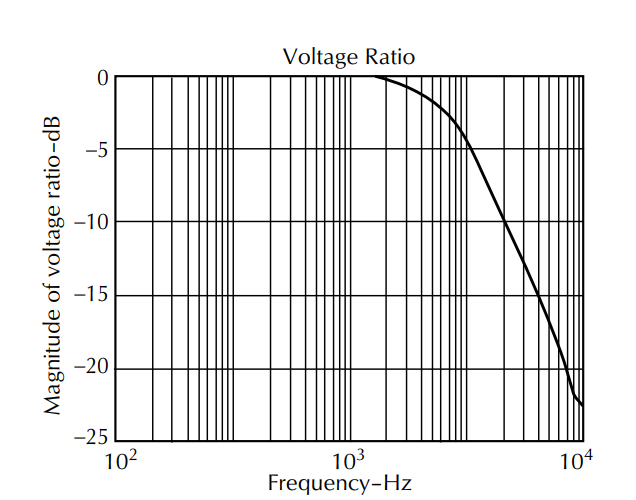
\includegraphics[width=%
0.50\textwidth]{lp}
\caption{Diagramma di Bode di un filtro passa basso \newline \scriptsize{ da D. Davis - Sound System Engineering - 2013}}
\label{fig:lp}
\end{figure}

\subsection{High-Pass}
Permette l’attenuazione delle frequenze inferiori alla frequenza di taglio.
La sua funzione di trasferimento è in figura \ref{fig:hp}

\begin{equation}
H(s)=\frac{st}{1+st}
\end{equation}

dove con $st$ indichiamo sempre la frequenza di taglio.
La risposta in frquenza ottenuta è la seguente
\begin{figure}[htp]
\centering
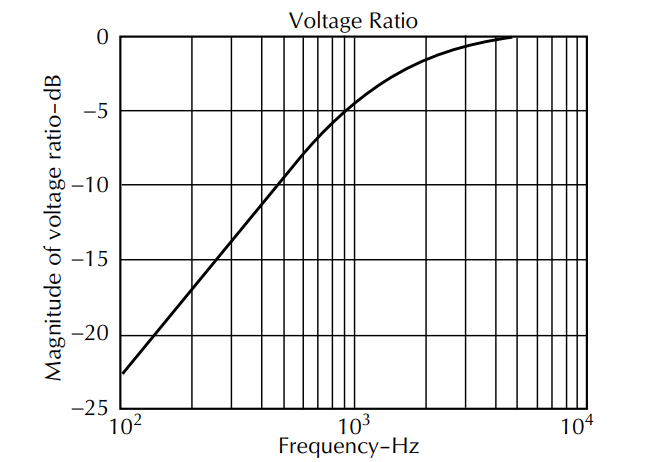
\includegraphics[width=%
0.50\textwidth]{hp}
\caption{Diagramma di Bode di un filtro passa alto}
\label{fig:hp}
\end{figure}

\subsection{Band-Pass}
Permette il passaggio solo ad una determinata banda di frequenze.
la sua funzione di trasferimento è la seguente
\begin{equation}
H(s)=\frac{(1+st_1)(1+st_4)}{(1+st_2)(1+st_3)}
\end{equation}
Considerando che $t_1>t_2>t3_>t_4$ e che il calcolo di poli e zeri risulta: $z_1=1/t_1$, $z_2=1/t_4$, $p1_=1/t_2$, $p_2=1/t_3$ \dots

La risposta in frquenza ottenuta è in figura \ref{fig:bp}
\begin{figure}[htp]
\centering
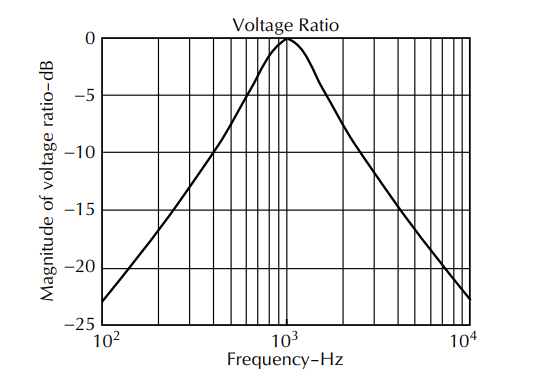
\includegraphics[width=%
0.50\textwidth]{bp}
\caption{Diagramma di Bode di un filtro passa banda}
\label{fig:bp}
\end{figure}


\section{Filtri Digitali}

Ovviamente tutto ciò che abbiamo visto fino a questo punto è puramente nel dominio continuo. Possiamo dunque procedere all’implementazione di tali modelli matematici in digitale. I filtri digitali utilizzano in larga scala algoritmi ricorsivi aventi al loro interno moltiplicazioni e addizioni, per i quali gli attuali strumenti informatici di cui disponiamo, sono ottimizzati. Definiamo 2 macro categorie di filtri digitali ovvero i cosiddetti filtri \textbf{FIR} e \textbf{IIR}.
\begin{itemize}
\item IIR: Infinite impulse response;
\item FIR: Finite impulse response.
\end{itemize}
Possiamo definire i filtri IIR come caratterizzati da una risposta all’impulso unitario non limitata (parlando di numero di campioni) e un’ampiezza tendente a zero.
Questo rende i filtri IIR molto simili alla loro controparte analogica (esistente nel tempo continuo).
Per quanto riguarda la loro composizione strutturale, notiamo generalmente una funzione di trasferimento costituita da un rapporto polinomiale, con poli e zeri. È esclusa una situazione in cui siano presenti soli zeri. Inoltre la costruzione di questi filtri prevede l’utilizzo di sistemi di feedback, e per questo, è risaputo che queste strutture hanno un comportamento instabile.

Parlando di filtri FIR, invece, possiamo affermare che la loro risposta all’impulso unitario è composta da un numero finito di campioni e per questo non associabili a nessun modello analogico.
A differenza dei filtri IIR, i filtri FIR, presentano una funzione di trasferimento a soli zeri.
Possedere una risposta all’impulso unitario limitata comporta, inoltre, una stabilità nell'implementazione, ma di conseguenza una necessità di maggiore potenza di calcolo.
(Lindoro del Duca - Musica Digitale - pag 85)

\section{Delay e Utilizzo}
Il \emph{Delay} è il ritardo temporale imposto ad un evento sonoro. Il Delay può essere percepito soltanto se messo in relazione ad un altro segnale, ovvero, il suono stesso ma non ritardato.
Questo fenomeno si manifesta in due situazioni: quando, in un ambiente riverberante il suono diretto raggiunge l’ascoltatore prima delle sue riflessioni, oppure quando, un delay elettrico, è volontariamente inserito per pareggiare due sorgenti sonore e simulare un’ unica provenienza.

Il delay è inoltre un componente chiave nella costruzione dei filtri digitali.
Nel dominio digitale, infatti, i singoli campioni di una sequenza vengono sottoposti a numerose operazioni (implicando un processo di quantizzazione) producendo una seconda sequenza di risultati che comporranno il segnale filtrato.
Le operazioni utilizzate sono: Somma, Prodotto e Delay (di un campione).
L’espressione che determina il comportamento del filtro è detta equazione differenza e, in base al numero di elementi di ritardo presenti, possiamo indicare l’ordine dell’equazione.

L’equazione differenza del primo ordine generale è definita secondo la seguente equazione:

\begin{equation}
Y(z)=A_0*x(z) + A_1*z^{-1}*x(z) + B_1*z^{-1}*y(z)
\end{equation}

L’equazione è scritta nel dominio z, con z detta frequenza complessa.
I valori di z che rendono rispettivamente nullo numeratore e denominatore vengono detti zeri e poli della funzione.

Tutte le equazioni differenza del primo ordine sono determinate dai coefficienti $A_0, A_1,B_1$.
Bisogna sempre considerare che un’equazione del primo ordine può descrivere solo un filtro passa basso o passa alto avente un’attenuazione di massimo 6 dB/ottava.

Partendo dall’equazione differenza, infine, possiamo ricavare la funzione di trasferimento $H(z)$ avente la seguente forma:

\begin{equation}
H(z)=\frac{(A_0 + A_1 * z^{-1})} {(1-B_1 * z^{-1})}
\end{equation}


L'implementazione di un riverbero artificiale non può che ripartire dale teorie
di \ms descritte in \ref{sec:schroeder1} che, oltre ad essere la prima
implementazione storica, costituisce l'unico momento di progettazione in cui
il rapporto hardware e software presenta problematiche uniche e fondamentali per
lo sviluppo del pensiero informatico.

Gli algoritmi sono stati scritti nel linguaggio \faust.

Sulle implementazioni dirette delle ricerche di \ms e \jam ho inserito il codice
necessario a controllare i parametri atmosferici quali temperatura, pressione e
tipologia del gas.

\clearpage
\section{Schroeder}

Con l’obiettivo di ricreare, passo dopo passo, le unità descritte nell’articolo
\emph{Natural Sounding Artificial Reverberation}\footcite{ms:rev62}, le prime
implementazioni in \faust~sono relative ai due blocchi essenziali, \emph{Comb}
e \emph{All-Pass}, e alle interazioni tra loro.

\subsection{Comb}

Il codice di studio del filtro \emph{Comb} descritto in fig. \ref{fig:dfl}, con
i passi di correzione del dei tempi di integrazione per l'ottenimento della
risposta all'impulso indicata da Schroeder e riportata in fig. \ref{fig:dflir}.

\lstinputlisting{Code/dflc.dsp}

\todo{sarebbe opportuno indicare le motivazioni della correzione del filtro}

Il l'algoritmo utilizza le variabili $t$ (unità di tempo di ritardo espressa in
campioni) e $g$ (coefficiente di riscalamento del segnale in feedback).

\begin{figure}[htp]
\centering
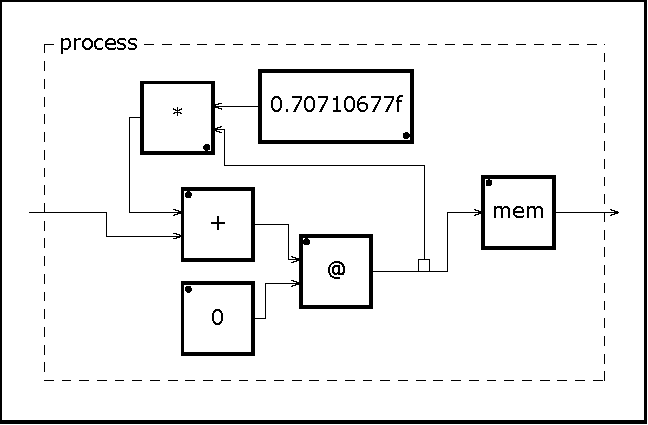
\includegraphics[width=0.80\textwidth]{Code/dflc-svg/process.pdf}
\caption{\emph{Delay Feedback Loop} con correzioni per l'implementazione
         digitale \emph{samplerate}: il modulo \emph{delay} opera un ritardo
         $t-1$ quindi con $t=1$ il ritardo accumulato internamente al ciclo di
         \emph{feedback} è $0$, il campione di ritardo per $x$ è recuperato dopo
         il ciclo di \emph{feedback}.}
\label{fig:dflfaust}
\end{figure}

\subsection{All-Pass}

Il secondo algoritmo implementato permette di ottenere un filtro All-Pass
con risposta impulsiva in frequenza e ampiezza identiche a quelle descritte
dall'autore con figura \ref{fig:apf}

\lstinputlisting{Code/msapf.dsp}

Il comportamento \emph{All-Pass} è dato dalla somma del segnale ritardato
scalato di $(1-g^2)$ e il segnale diretto per $-g$, scalato con inversione di
polarità.

\begin{figure}[htp]
\centering
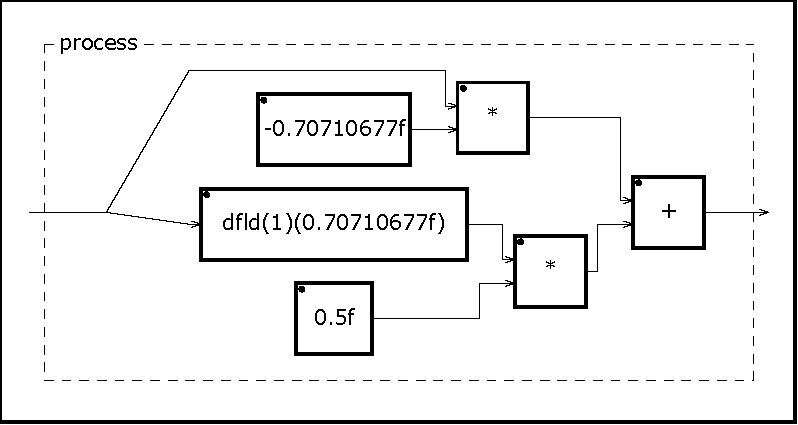
\includegraphics[width=0.80\textwidth]{Code/msapf-svg/process.pdf}
\caption{\emph{All-Pass}}
\label{fig:apfaust}
\end{figure}

\subsection{Sequenza di All-Pass}

I filtri \emph{Comb} e \emph{All-Pass} implementati sono gli elementi basilari
della riverberazione artificiale di \ms. Di seguito espongo le implementazioni
articolate, dei filtri sopra descritti, che l'autore espone.

\lstinputlisting{Code/msapfseq.dsp}

\begin{figure}[htp]
\centering
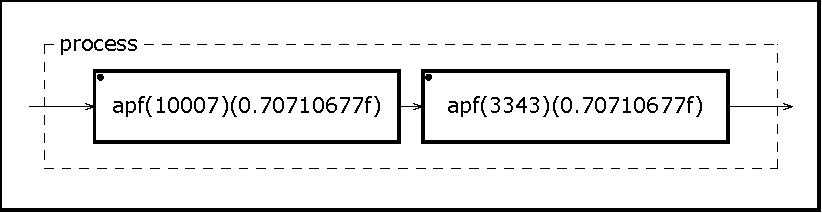
\includegraphics[width=0.80\textwidth]{Code/msapfseq-svg/process.pdf}
\caption{Sequenza di \emph{All-Pass}}
\label{fig:apfseq}
\end{figure}

\subsection{Annidamento e controllo}

\ms, immediatamente dopo la creazione degli elementi base, espone una serie di
risultati sperimentali ottenuti nella ricerca della simulazione di alcuni dei
comportamenti del riverbero acustico. Uno di questi è la possibilità di annidare
un \emph{All-Pass} dentro un \emph{All-Pass} in modo che i due filtri combinati
possano:
\begin{enumerate}
  \item bilanciare il rapporto tra segnale diretto e segnale riverberato
  \item l'introduzione di un ritardo tra i due segnali (diretto e riverberato)
  \item una dipendenza del tempo di riverberazione dalla frequenza
\end{enumerate}

\lstinputlisting{Code/msapfdwp.dsp}

\begin{figure}[htp]
\centering
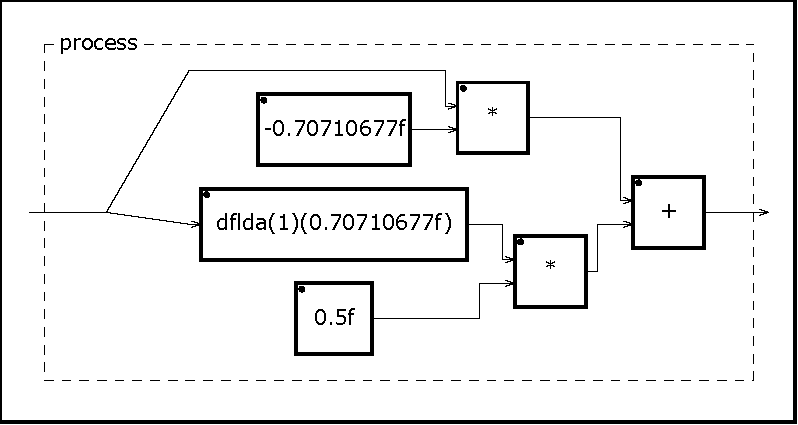
\includegraphics[width=0.80\textwidth]{Code/msapfdwp-svg/process.pdf}
\caption{All-Pass contenente una unità comb contenente una unità all-pass}
\label{fig:apfdwp}
\end{figure}

\begin{figure}[htp]
\centering
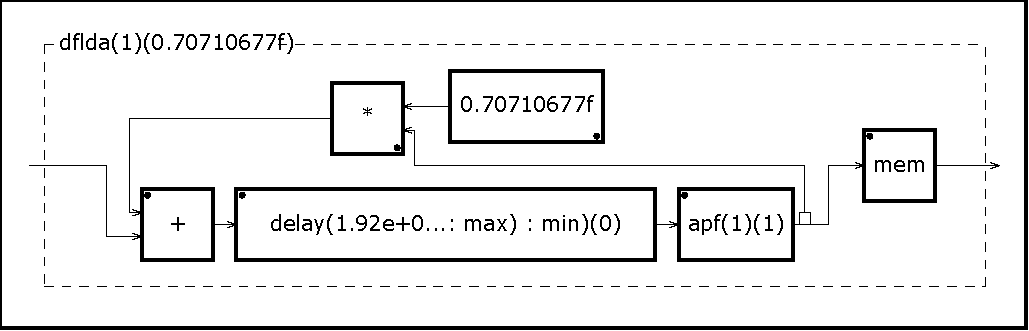
\includegraphics[width=0.80\textwidth]{Code/msapfdwp-svg/dflda-0x600001c847e0.pdf}
\caption{dfla: unità comb contenente un all-pass}
\label{fig:dfla}
\end{figure}

\subsection{Algoritmi Combinati}

Come già visto nel Capitolo 3, \todo{rifare puntatore al paragrafo corretto}
queste unità riverberanti, prese singolarmente, non risultano particolaremente
efficaci dal punto di vista della densità. Il passo successivo è quindi quello
di crare delle reti di riverberatori combinando queste unità fondamentali.

\lstinputlisting{Code/mscombapf.dsp}

\begin{figure}[htp]
\centering
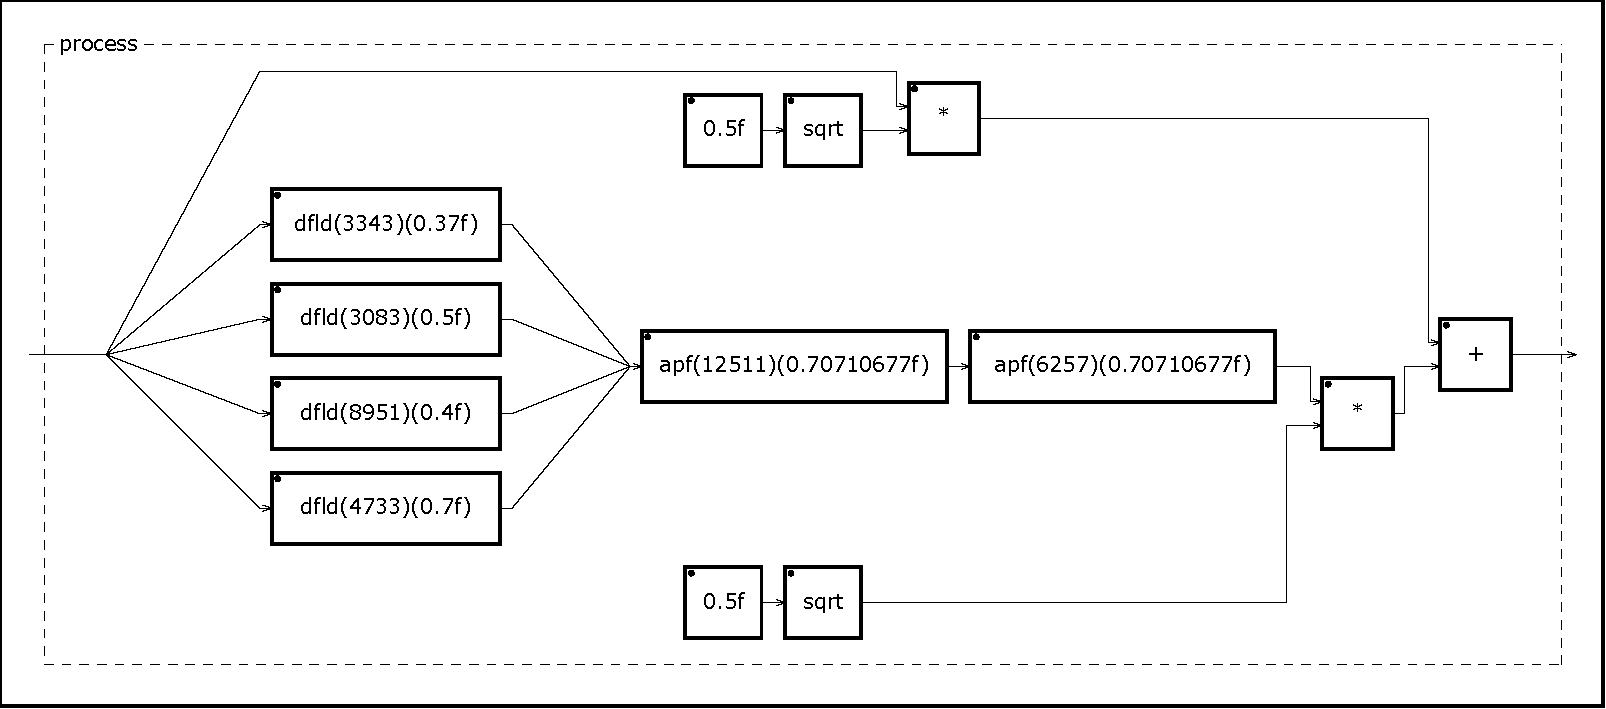
\includegraphics[width=1\textwidth]{Code/mscombapf-svg/process.pdf}
\caption{Modello di riverberatore complesso di Schroeder: Filtri Comb in parallelo
         in filtri All-Pass in serie}
\label{fig:mscombapf}
\end{figure}

Quest'algoritmo risulta essere il più efficace ad ora e permette la
riproduzione di oltre $1000$ echi al secondo, un buon risultato considerando
le stime effettute da Schroeder, ma che non corrisponde ad una riverberazione
realistica e gradevole.

\lstinputlisting{Code/msapfcomb.dsp}

\todo[inline]{dovresti scrivere che il capovolgimento del flusso di elaborazione del
segnale non produce comportamenti differenti ed il riverbero calcolato è identico.
il sistema capovolto permette però la generazione di un segnale polifonico}

\begin{figure}[htp]
\centering
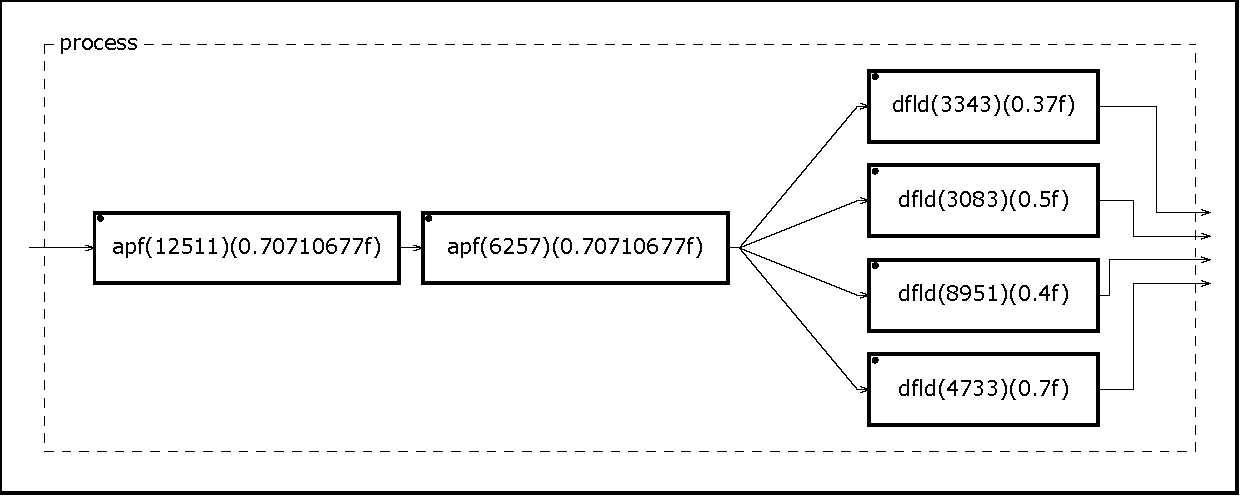
\includegraphics[width=1\textwidth]{Code/msapfcomb-svg/process.pdf}
\caption{Modello capovolto}
\label{fig:msapfcomb}
\end{figure}

\clearpage
\section{Algoritmi di Moorer}

In seguito alla fase di test, il passo successivo è stato quello di implementare gli algoritmi di Moorer, in quanto risultano più efficenti dei precedenti.
In questa sezione verranno inoltre inseriti i parametri ambientali ed utilizzati come controllo delle caratteristiche del riverbero. Le formule utilizzate per il calclo dei parametri sono le medesime viste nel capitolo \ref{chp:Filtri} ma con le dovute approssimazioni.

\bigskip

Il codice seguente descrive il filtro All Pass secondo le indicazioni di Moorer (visto in figura \ref{fig:apfmoorer}) e come già detto, senellisce i calcoli riducendo il numero delle moltiplicazioni ad 1.

\begin{code}
apfm(t, g) = _<: ((+ : _*(g)),_<:_,!,_+_ : _, zm(t) : ro.cross(2))~(0 -_) : +
with{
    zm(t) = de.delay(ma.SR,t);
};
\end{code}

\bigskip

Il grafico risultante è in figura \ref{fig:apfmoorerfaust}

\begin{figure}[htp]
\centering
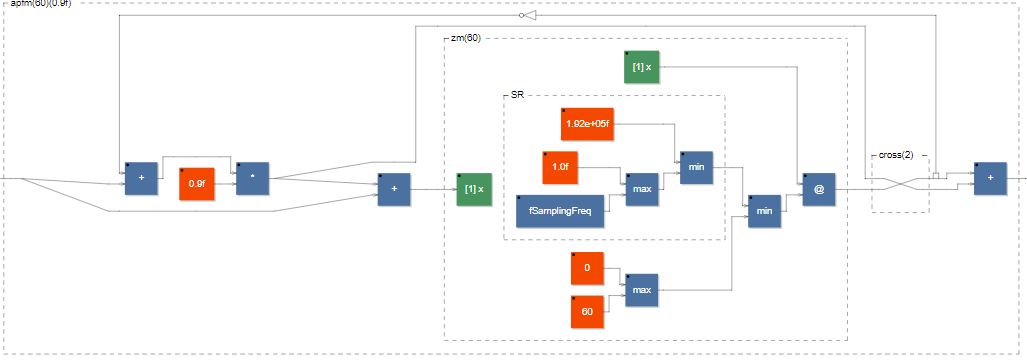
\includegraphics[width=%
1.2\textwidth]{apfmoorerfaust}
\caption{All Pass descritto da Moorer}
\label{fig:apfmoorerfaust}
\end{figure}


%\input{Chapters/Cap3}
%% !TEX TS-program = pdflatex
% !TEX root = ../tesi.tex

%************************************************
\chapter{Implementazione}
\label{chp:Implementazione}
%************************************************

In questo capitolo sarà presente l’analisi degli algoritmi che compongono il sistema riverberante creato. Gli algoritmi sono stati scritti nel linguaggio Faust sulla base delle ricerche svolte da Schroeder e Moorer e presentano le dovute modifiche che rispecchiano l’idea iniziale, vale a dire utilizzando parametri quali temperatura, pressione e tipologia del gas per variare la risposta del riverbero.

\section{Algoritmi di Schroeder}

I primi algoritmi sono stati creati partendo dalle soluzioni ottenute da Schroeder e utilizzati a scopo di test. L’obiettivo è stato quello di ricreare passo dopo passo le unità descritte nell’articolo Natural Sounding Artificial Reverberation. 

\subsection{Algoritmi fondamentali}

Partendo quindi dagli elementi fondamentali, abbiamo, come primo sistema il filtro Comb descritto in \ref{fig:dfl}.
\begin{code}
dfld(t, g) = ( + : de.delay(ma.SR,t-1))~(*(g)) : mem; //delay feed loop 
process = os.impulse : dfld(1000,.707);
\end{code}

Il codice presenta le variabili t e g che rappresentano rispettivamente il numero di campioni di ditardo e il moltiplicatore del feedback.
La funzione de.delay è utilizzata per il ritardo di un determinato numero di campioni.
Il simbolo \verb!~! permette l'utilizzo di una recursione, ovvero divide il segnale inviando una sua copia all'entrata del processo, creando \emph{feedback}
Il diagramma di questo codice è in figura \ref{fig:dflfaust}.

\bigskip

\begin{figure}[htp]
\centering
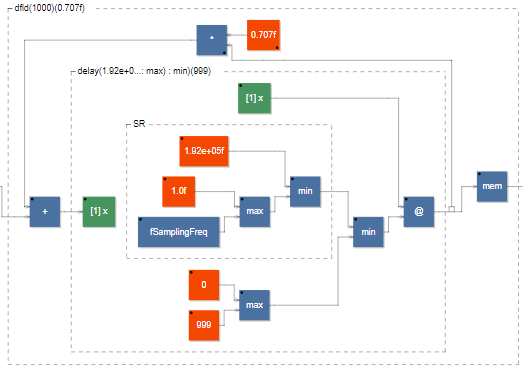
\includegraphics[width=%
0.80\textwidth]{dflfaust}
\caption{delay feedback loop}
\label{fig:dflfaust}
\end{figure}

Il secondo algoritmo derivato permette di realizzare un filtro All Pass, come quello descritto in figura \ref{fig:apf}

\begin{code}
apf(t,g) = _ <: *(-g) + (dfld(t,g)*(1-g^2));
process = os.impulse : apf(1,.71);
\end{code}

Il comportamento All Pass è dato dalla somma del segnale ritardato moltiplicato per $(1-g^2)$ e il segnale diretto moltiplicato per $-g$
Il diagramma di questo codice è in figura \ref{fig:apfaust}.

\begin{figure}[htp]
\centering
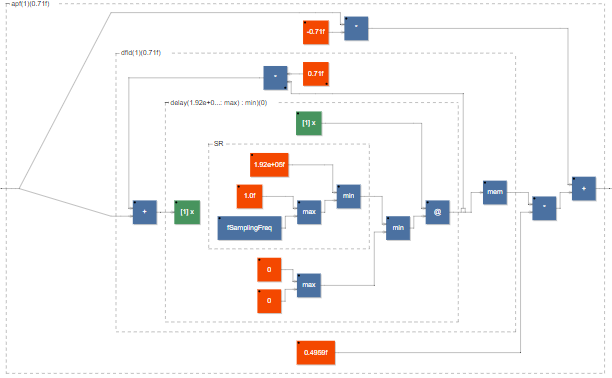
\includegraphics[width=%
0.90\textwidth]{apfaust}
\caption{All Pass}
\label{fig:apfaust}
\end{figure}

\subsection{Algoritmi derivati}

I prossimi algoritmi sono i successivi descritti da Schroeder. Presentano una serie di miglioramenti che auspicano ad una maggior naturalezza nella risposta del filtro. 
Come abbiamo visto in figura \ref{fig:apfmix}, creiamo un All Pass contenente un secondo All Pass e un delay al suo interno, per simulare il ritardo che intercorre tra il suono diretto e il suono riverberato.

\smallskip

il nuovo All Pass è dunque:
\begin{code}
dflda(t,g) =  (+ : de.delay(ma.SR,t-1) : apf(t,g))~ *(g) : mem;
\end{code}

Il suo diagramma lo troviamo in figura \ref{fig:dfldafaust}

\begin{figure}[htp]
\centering
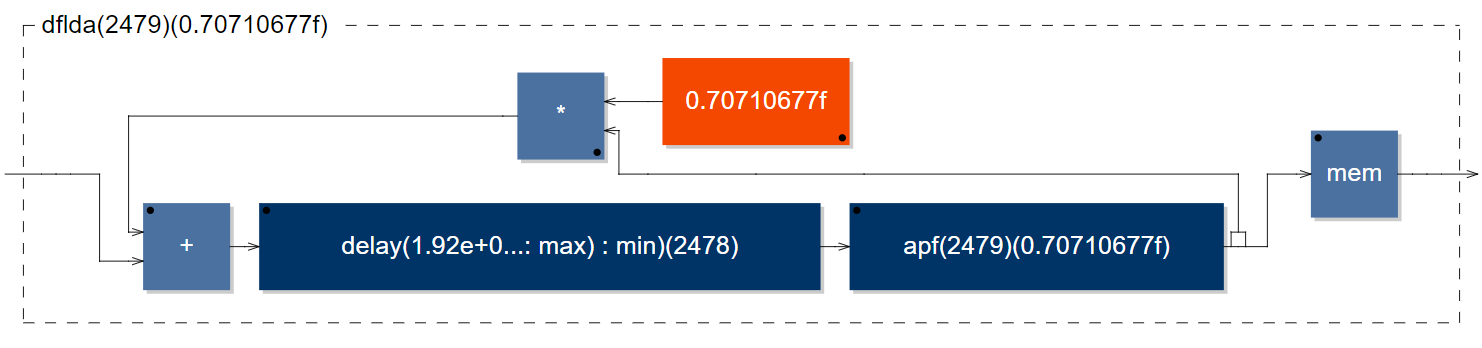
\includegraphics[width=%
0.90\textwidth]{dfldafaust}
\caption{Nuovo All Pass}
\label{fig:dfldafaust}
\end{figure}

Dato che abbiamo la necessità di missare il risultato del precedente filtro con il segnale diretto, creiamo un secondo ogetto che ci permette di farlo.

\begin{code}
apfn(t,g) = _ <: *(-g) + dflda(t,g) * (1-g^2);
\end{code}

\begin{figure}[htp]
\centering
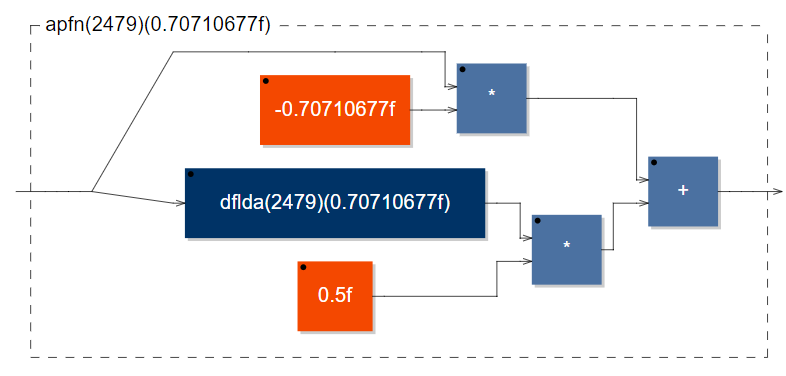
\includegraphics[width=%
0.70\textwidth]{apfmixfaust}
\caption{Nuovo All Pass con mix segnale diretto}
\label{fig:apfmixfaust}
\end{figure}

Il valore di g, inoltre, permette di decidere la quantità di segnale riverberato che vogliamo, come se fosse un pomello `'Dry/Wet''.

\subsection{Algoritmi Combinati}
Come già visto nel Capitolo 3, queste unità riverberanti non risultano particolaremente efficenti dal punto di vista della densità, se prese singolarmente, quindi il prossimo passo, come suggerito da Schroeder, è quello di crare delle reti di riverberatori combinando queste unità fondamentali.

\bigskip

Le due tipologie proposte consistono in una serie di All Pass connessi (figura \ref{fig:apfseq}), per la prima e, una serie di Comb connessi in cascata seguiti da 2 All Pass in serie, per la seconda.
Durante questa fase sono stati utilizzati numeri primi come valori dei ritardi in modo da evitare errori dovuti al campionamento.

L'algoritmo per la configurazione in serie risulta essere

\begin{code}
apfseq =  seq(i, 5, apf(ba.take(i+1, primet10),.7));
\end{code}

La lista ''primet10'' è stata caricata con i valori dei vari t. Come suggerito dall'autore, si è cercato di utilizzare numeri primi che mantenessero una relazione di $1/3$ l'uno dall'altro.
Il diagramma risultante è in figura \ref{fig:apfseqfaust}.

\begin{figure}[htp]
\centering
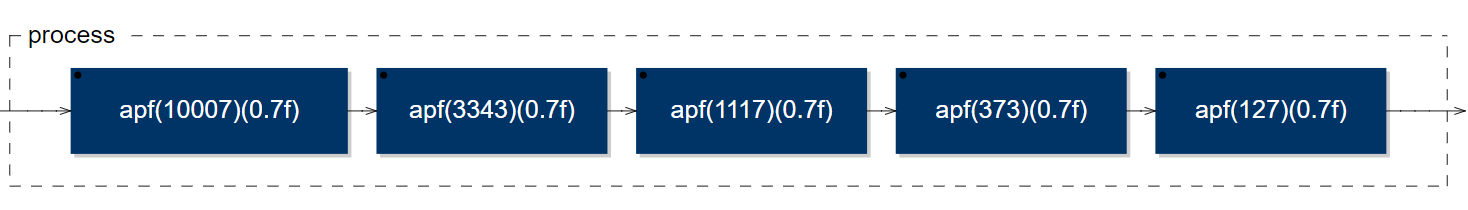
\includegraphics[width=%
0.90\textwidth]{apfseqfaust}
\caption{Sequenza di All Pass}
\label{fig:apfseqfaust}
\end{figure}

Il secondo algoritmo, per la configurazione `'Comb-All Pass'' vista in figura \ref{fig:comballpass}, è descritto nel seguente algoritmo

\begin{code}
reva((t,g,t1,g1),g2) = _<:_+(
    par(i,6, dflda(ba.take(i+1, t),G*ba.take(i+1,g))) :> 
    seq(i, 2, apfn(ba.take(4-i, t1),G*ba.take(i+1,g1))))*(g2);
process = _ : reva((primetc1,combg1,primetc2,combg2),G);
\end{code}

`'par'' e `'rev'' sono rispettivamente, composizione parallela e composizione sequenziale e ci permettono di creare una cascata di 6 Comb seguita da una sequenza di 2 All Pass. 

Il risultato è in figura \ref{fig:comballpassfaust}.

\begin{figure}[htp]
\centering
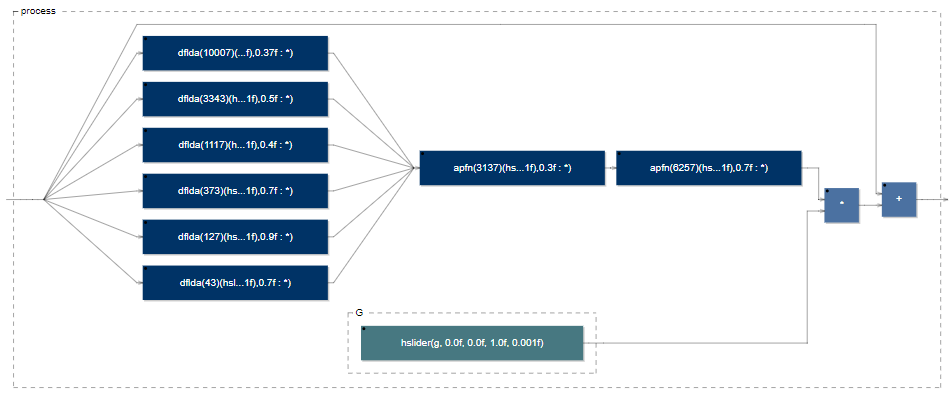
\includegraphics[width=%
1.2\textwidth]{comballpassfaust}
\caption{Algoritmo Comb-All Pass}
\label{fig:comballpassfaust}
\end{figure}

Quest'algoritmo risulta essere il più efficente ad ora e permette la riproduzione di oltre 1000 echi al secondo, un buon risultato considerando le stime effettute da Schroeder, ma che non corrisponde ad una riverberazione realistica e gradevole.

\section{Algoritmi di Moorer}

In seguito alla fase di test, il passo successivo è stato quello di implementare gli algoritmi di Moorer, in quanto risultano più efficenti dei precedenti. 
In questa sezione verranno inoltre inseriti i parametri ambientali ed utilizzati come controllo delle caratteristiche del riverbero. Le formule utilizzate per il calclo dei parametri sono le medesime viste nel capitolo \ref{chp:Filtri} ma con le dovute approssimazioni.

\bigskip

Il codice seguente descrive il filtro All Pass secondo le indicazioni di Moorer (visto in figura \ref{fig:apfmoorer}) e come già detto, senellisce i calcoli riducendo il numero delle moltiplicazioni ad 1.

\begin{code}
apfm(t, g) = _<: ((+ : _*(g)),_<:_,!,_+_ : _, zm(t) : ro.cross(2))~(0 -_) : +
with{
    zm(t) = de.delay(ma.SR,t);
};
\end{code}

\bigskip

Il grafico risultante è in figura \ref{fig:apfmoorerfaust}

\begin{figure}[htp]
\centering
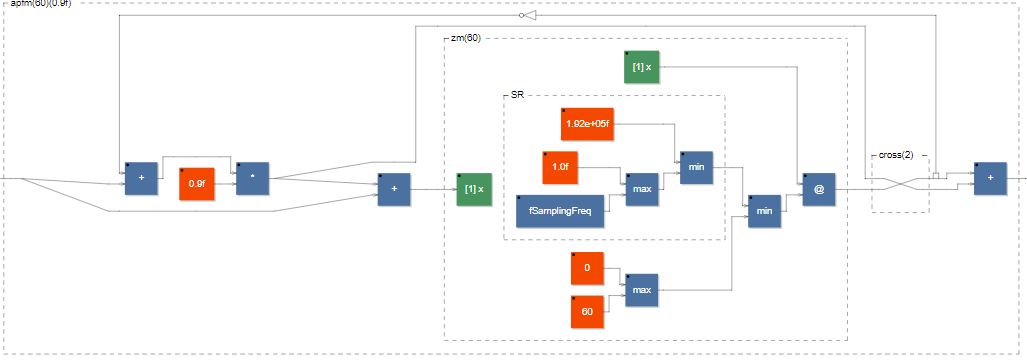
\includegraphics[width=%
1.2\textwidth]{apfmoorerfaust}
\caption{All Pass descritto da Moorer}
\label{fig:apfmoorerfaust}
\end{figure}

% !TEX TS-program = pdflatex
% !TEX root = ../tesi.tex

%************************************************
\chapter{Conclusioni}
\label{chp:Conclusioni}
%************************************************
Sulla base dei risultati ottenuti nel capitolo \ref{chp:Implementazione}, possiamo trarre alcune
considerazioni sul lavoro svolto.
Certo, si può affermare senza dubbio che le condizioni atmosferiche hanno una certa
influenza sul risultato riverberante; sia il tempo che il carattere di riverberazione, infatti, hanno un
risultato differente in base ai parametri che si vanno man mano modulando. I risultati sonori
non sono certo eccezionali, se consideriamo il tutto da un punto di vista prettamente scientifico.
Certamente non ci troviamo di fronte ad una rappresentazione fedele della realtà date le numerose
approssimazioni ma, dal punto di vista espressivo, delle potenzialità mi sento di vedercele. A fronte
del lavoro svloto, dei risultati e in generale dell'esperienza ottenuta svolgendo questa tesi,
posso tranquillamente affermare di trovarmi di fronte un buon punto di partenza per ulteriori
miglioramenti e approcci diversificati per raggiungere l'obiettivo.

\todo[inline]{credo tu abbia confuso il ruolo del paragrafo conclusivo. non si
tratta di dare giudizi soggettivi o considerazioni personali. Si trtta di riprendere
gli argomenti aperti con l'introduzione e concludere il cerchio spiegando cosa
ha porta a cosa e con quali caratteristiche e corrispondenze. Per esempio:

il presupposto di controllare un riverbero artificiale ha dato risultati difficilmente
ottenibili con i parametri tradizionali?

il controllo parametrico ambientale è qualcosa che fa relazionare con lo strumento
riverbero in modo diverso dai parametri tradizionali? perchè?

inoltre, dato che tu non inventi un nuovo riverbero ma utilizzi riverberi storici
per mettere a punto la matematica ambientale, non ha senso parlare di bellezza del
riverbero}

\clearpage
\addcontentsline{toc}{chapter}{Indice dei nomi}
\printindex[names]
\input{FrontBackMatter/Bibliography}
\end{document}
